% !TEX TS-program = xelatex
\documentclass[12pt]{article}

\usepackage[margin=2cm]{geometry}
\usepackage{colortbl}
\usepackage{comment}
\usepackage{caption}
\usepackage{subcaption}
\usepackage{mathptmx}
\usepackage{nicefrac}
\usepackage{authblk}

\usepackage{times}
\usepackage{lineno}
\usepackage[round]{natbib}
\makeatletter
\renewcommand{\@biblabel}[1]{#1.}
\makeatother

\usepackage{graphicx}
\usepackage{amsmath}
\usepackage{xcolor}

\usepackage{url}
\urlstyle{same}

\usepackage[small,compact]{titlesec}

%\titleformat{\section} {\vspace{24pt}\bf\sffamily\MakeUppercase}{\thesection} {0pt} {}
\titleformat{\section} {\vspace{12pt}\bf\large}{\thesection}{0pt}{}
\titleformat{\subsection} {\vspace{6pt}\bf}{\thesubsection} {0pt} {\vspace{-2pt}}
\titleformat{\subsubsection} [runin] {\bf}{\thesubsubsection} {12pt} {}

\definecolor{badpatcol}{HTML}{FF6666}
\newcommand{\badpat}[1]{\rowcolor{badpatcol}#1}

\captionsetup[subfigure]{width=0.9\textwidth}

\newcommand{\high}[1]{{\textcolor{badpatcol} #1}} 
 
\begin{document}

\title{Blind dating: A phylogenetic approach to dating HIV reservoir sequences}

\author[1,2]{Bradley R. Jones}
\author[1,2]{Joshua Horacsek}
\author[1,3]{Jeffrey B. Joy}
\author[1,2]{Zabrina L. Brumme}
\author[1,2,3]{Art F.Y. Poon}
\affil[1]{Simon Fraser University, Burnaby, Canada}
\affil[2]{BC Centre for Excellence in HIV/AIDS, Vancouver, Canada}
\affil[3]{University of British Columbia, Vancouver, Canada}
%%% 1 Simon Fraser University
%%% 2 BC Centre for Excellence in HIV/AIDS
%%% 3 University of British Columbia
\baselineskip 22pt
\pagewiselinenumbers

\date{}
\maketitle

\section * {Abstract}

%Background: 
The ability of HIV to persist within latent cellular reservoirs represents a major barrier to developing an effective cure.
The timing of establishment of individual viral reservoirs over the course of an infection may influence their susceptibility to elimination by immune-mediated or therapeutic approaches.
However, methods to accurately estimate the age of reservoir sequences remain scarce.
We propose a simple method to date suspected reservoir sequences using phylogenetically informed regression.

%Method: 
%Simulated sequence data were generated.
%A total of 410 HIV RNA sequences sampled longitudinally from 9 untreated HIV-infected individuals with estimated dates of infection and a total of 2816 HIV DNA and RNA sequences from 20 individuals were obtained from the Los Alamos National Laboratory HIV Sequence Database.
%The simulated and HIV RNA data were used for method validation.
Our method is as follows: Taking aligned HIV sequences from a single individual sampled over multiple time points, we reconstruct a maximum-likelihood phylogeny.
The phylogeny is rooted by determining the location of the root using root-to-tip regression.
The root-to-tip distances of possibly latent sequences are mapped to the optimal regression line to estimate reservoir establishment dates.
Finally a nonparametric binary test is applied amongst multiple individuals to identify the presence of latent lineages.

To validate our method, we generated simulated HIV sequences and used RAxML to infer phylogenies from the simulated HIV sequences.
We then applied our method to simulated sequences with and without latency and to HIV RNA datasets.
Next we simulated latent lineages by shortening tip lengths and employed the same methodology as above.
%We synthesized latent lineages by censoring the sample dates for random selections of up to 50\% of sequences in the simulated and HIV RNA datasets.
When this method was applied to HIV DNA sequences in phylogenies containing dated HIV RNA sequences, we observed that the predicted dates tended to precede dates of sampling, consistent with latency.

Our results indicate that the dates when HIV DNA lineages entered a latent state can be accurately estimated from a phylogenetic analysis of HIV RNA sequence variation from the same patient.
This can provide important insights into the dynamics of HIV reservoirs within hosts.


Keywords: 
HIV, Latency, Cellular Reservoirs, Phylogenetics, Linear Regression\\



\underline{}
\section * {Introduction} \label{sec:intro}

A major obstacle in developing HIV cure strategies is the long-term persistence of the virus within latently infected cellular reservoirs \citep{Pace11}. 
Latently infected cells contain integrated HIV DNA and have entered a dormant state in which they not only have a lowered rate of virion production, but may also persist within an individual for several years or more.
Although a patient's viral load can be reduced below detectable levels when that patient is subjected to highly active antiretroviral therapy (HAART), latent reservoirs will eventually reseed an infection if a patient halts treatment \citep{Joos08, Pomerantz03, Richman09}. 
Not much is known about when specific latent reservoirs are established over the course of an infection. 
The chronology of their establishment is of interest as the distribution of ages of the latent virus lineages may provide information concerning the types of adaptations that those lineages may have accumulated. 
Specifically, the timing of reservoir establishment may influence how virions produced by those reservoirs will react to immune-mediated and/or therapeutic treatments. 
Previous studies have developed techniques to detect latent lineages by reduced rates of viral evolution \citep{Immonen14} and modeled the population dynamics of different classes of the virus within host \citep{Althaus14}. 
However, there has been limited research on estimating when viral lineages suspected of being latent became integrated into the host genome, or qualitatively assessing the distribution of collection-age differences for suspected latent samples.

An HIV-1 population rapidly accumulates genetic diversity over the course of an infection, due to its high mutation rate and short generation time %, and intense selective pressure by the host's immune system 
\citep{Alizon13, Shankarappa99, Rambaut04}. 
Using this extensive sequence diversity, it is possible to reconstruct a phylogenetic tree that represents the descent of virus lineages that have been sampled from a given infection from their common ancestors. 
A phylogeny that is reconstructed by parameterizing a model of molecular evolution \cite[\textit{e.g.}, by maximum likelihood estimation;][]{Felsenstein:1981} solely on the basis of sequence homology has branch lengths in units of expected numbers of substitutions, in which the passage of time is confounded with the rate of evolution.
In other words, a tree that stretches far back in time with a slow rate of evolution will explain a given set of sequences just as effectively as a shallow tree with rapid evolution.  
When lineages are known to be sampled at different times, however, the corresponding tips of the phylogeny can be fixed in time and the rate of evolution between the tips can be estimated directly \citep{Rodrigo99}.
This additional information enables one to rescale a phylogeny in chronological time, which is especially true for HIV-1 populations in which genetic differences can accumulate in weeks or months \citep{Williamson:2003}.
%With an appropriate method of relating evolutionary distance to time (a {\em clock model}), the phylogeny can be re-scaled chronologically, then by fixing the tips to their respective sampling dates, clock ``rates'' can be estimated .
Among the actively replicating HIV lineages within a host, the rate of molecular evolution is fairly consistent over time \citep{Leitner99, Kuhner95, Korber00}.
Consequently, the initial divergence of these lineages from the transmitted/founder virus can be adequately approximated by a `strict' molecular clock model in which a single rate of evolution is sustained throughout \citep{Keele08}.
%For sequences originating from the active population of virus, it is not unreasonable to assume that the rate of molecular evolution is relatively constant --- in other words, it adheres to a `molecular clock' model . 
Once a virus lineage becomes integrated into a host genome, however, its rate of evolution becomes negligible relative to the baseline rate in the actively replicating population.
Thus, viral latency effectively halts the molecular evolution of that particular virus lineage until reactivation. 

%Between the active and latent populations, latent cells are then expected to be more genetically different to active lineages than active lineages are among each other.

Viral latency can be manifested by discordance between a sample's actual collection time and its apparent age based on its sequence divergence from other lineages (Figure \ref{fig:latenttree}). 
Therefore, it may be possible to use phylogenetic analysis to recover the dates that a given virus lineage became latent.
We propose a simple framework to estimate dates of latent reservoirs which assumes that HIV evolution within a host can be adequately modeled by a strict molecular clock, such that the expected number of substitutions per site increases linearly with time \citep{Ho14}. 
%Our method extracts timing information from the phylogenetic relationships between the virus sampled at various time-points along the infection. 
First, we construct a phylogeny relating sequences derived from both cellular HIV DNA and plasma HIV RNA sampled from the same patient.
Next, we parameterize a strict clock by fitting a linear model to the known collection dates of the HIV RNA sequences and the path lengths from the corresponding tips of the phylogeny to the root, which represents the earliest point in time in the phylogeny. 
Since phylogenies reconstructed by the comparative analysis of sequences are typically unrooted, we employ both root-to-tip regression \citep{Korber00} and outgroup rooting methods to estimate the location of the root in the tree. 
We assume that sequences derived from cellular HIV DNA such as that extracted from peripheral blood mononuclear cells (PBMCs) are potentially derived from latent reservoirs. %, and therefore have effectively stopped evolving.
Although sequences derived from plasma HIV RNA may potentially be descended from reactivated latent virus lineages, we assume that this affects only a minority of sequences derived from blood plasma on the time scales represented by the longitudinal data sets in our study (see below).
We used simulated and real longitudinal HIV sequence data sets to evaluate the accuracy of reconstructing tip dates by this approach.
Finally, we applied our method to characterize the integration dates of viral lineages sampled as cellular HIV DNA.

%
%Next, we evaluated the same model on sequence data that was simulated under a model that included viral latency in the form of a variable molecular clock.
%To mimic the types of results we expected from our first test, we used a collection of published longitudinal patient-derived sequence data sets comprising exclusively plasma-derived HIV sequences \citep{McCloskey14} to evaluate the accuracy of date reconstruction for sequences with censored dates. 
%Finally, we tested our methodology on another collection of longitudinal patient-derived data sets comprising both PBMC and plasma sequences. 
%If the molecular clock assumption holds for all sequences, and latency merely implies a ``pause'' in the evolution of a sequence, then the clock should be a reliable source of information for dating latent sequences.




%%%%%%%%%%%%%%%%%%%%%%%% METHODS %%%%%%%%%%%%%%%%%%%%%%%%%%

\section * {Methods} \label{sec:methods}



\subsection * {Data Collection} \label{subsec:dcollection}
We collected two distinct sets of data for our experiments. 
The first we refer to as the {\em plasma} data set, which comprised over 19,000 published HIV \textit{env} sequences derived from viral RNA from longitudinal plasma samples ($n=335$) collected from 232 different individuals \citep{McCloskey14}. 
From these data, we selected treatment naive individuals with two or more clonal or single-genome sequences available at each time point, and with a known time-line relative to one of several reference points: HIV infection, seroconversion or presentation of symptomatic seroconversion illness. 
The baseline samples were collected within 186 days of this reference point, and at least one of the subsequent ``follow-up'' time points occurred a minimum of 6 months after baseline.
Individuals who had been classified as ``superinfected'' were also excluded \citep{McCloskey14}.
After applying these criteria, we retained 410 HIV RNA sequences from 9 individuals for phylogenetic analysis.
The purpose of the plasma data set was to provide representative samples of within-host HIV diversity for evaluating and calibrating the model.

The second data set, referred to as the {\em mixed} data set, contained sequences from studies in which both plasma HIV RNA and cellular HIV DNA had been collected from the same individual.
We used the Los Alamos advanced search interface \citep{LosAlamos} to identify published data sets representing individuals with both HIV RNA and cellular DNA sequences.
%% what do you mean by "well-characterized"?
From these results, we manually selected 20 individuals that had well-characterized partial {\em env} sequences and plasma samples from at least 2 RNA time points and 3 DNA time points. 
%We also required that at least 1 RNA time point fell between 2 DNA time points in each individual
Other than this there were no selection criteria on the time between sample collection dates. 
A total of 1,017 partial {\em env} sequences from blood plasma, and 1,799 partial {\em env} sequences from PBMC cells were used in our analysis. 
We utilized samples from treatment naive individuals from \cite{Shankarappa99, Novitsky09} and samples from individuals that had been intermittently treated via HAART from \cite{Llewellyn06,Fischer04}. 

See Table \ref{tab:patients} for details on the patients from these data sets.

\subsection * {Sequence Alignment} \label{subsec:seqalign}
When applicable, we used MUSCLE 3.8.31 \citep{Muscle04} to align the patient-derived sequences, which were then visually inspected and cleaned with AliView \citep{AliView14}. 
Alignments were manually trimmed to the interval in which at least  50\% of sequences within the data set had coverage over each base.
%Since the simulated sequence data contained no insertions or deletions, no alignment of these data was necessary. 
The {\emph plasma} data set had already been aligned and cleaned \citep{McCloskey14}, so no further alignment was performed.

\subsection * {Simulated Data} \label{subsec:simdata}

%%% 1. simulate trees with strict clock - baseline
%%% 2. directly manipulate plasma trees
%%% 3. simulate sequence evolution on trees - additional error

To characterize sources of error in reconstructing dates on tips of a phylogeny, we generated phylogenetic trees by direct simulation. % and from the plasma data sets.
First, we generated phylogenies with 100 tips each under a birth-death model with serial sampling using the \emph{sim.bdsky.stt} function in the \textit{R} package \textit{TreeSim} \citep{Boskova14}.
Birth-death models have been applied to studying speciation processes \citep{Nee:2006} and infectious disease epidemics \citep{Stradler13}, but have only recently been used to model the proliferation of virus lineages in cell populations \citep{Hartfield:2015}.
%% This paragraph needs to be rewritten
The birth-death model was parameterized by fitting this model to samples from the {\em plasma} dataset.
%% we may need to provide some justification for using BD
%To assess the sensitivity of our method, we first simulated HIV sequence data sets without viral latency.
We used BEAST version 2.3.2 to estimate the posterior distribution defined by the serial model with a Bayesian skyline, a strict molecular clock, and the HKY85 \citep{HKY85} model of nucleotide substitution.
%Using this approach, we generated samples of trees for each sequence alignment in the plasma dataset.
%From these simulations, we evaluated the accuracy of predicting sample collection times from a strict molecular clock model that was fit to a training subset of these data.
The lineage birth rate, death rate and sampling probability were estimated to be: $\lambda = 5.116 \times 10^{-2}$ day$^{-1}$, $\delta = 5.006 \times 10^{-2}$ day$^{-1}$, $s = 5.237 \times 10^{-3}$ respectively.

We used the \textit{R} package, \emph{NELSI} \citep{NELSI}, to assign rates of evolution to these trees by drawing values from a Gaussian distribution with a mean rate $\mu = \ 1.964\times 10^{-4}$ substitutions per generation and standard deviation $\sigma = \ 1.417\times 10^{-5}$. %; Figure \ref{fig:seedtree} for an example).

To model uncertainty in phylogenetic reconstruction from sequence variation, we simulated sequence evolution along each birth-death tree with INDELible version 1.03 \citep{Indelible09} under an HKY85 \citep{HKY85} model of nucleotide substitution.
Parameters for the substitution model were set to empirical estimates derived from previously published HIV within-host data sets \citep{McCloskey14}. 
Specifically, the stationary distribution was set to 0.42, 0.15, 0.15, 0.28 for the nucleotides A, C, G and T, respectively, and the transition bias parameter was set to 8.5. Using this approach, we generated a total of 50 replicate subjects without viral latency. 

%A phylogeny was reconstructed from the simulated sequence alignments using the approximate maximum likelihood heuristic implemented in FastTree2.
%Similar results were obtained with trees reconstructed using RAxML \citep{Raxml14}, which is expected to be more accurate, but can consume orders of magnitude more computational time.

To simulate phylogenies with latent viral lineages, we employed an approach similar to  \citet{Immonen14}. 
However, we used the simplifying assumptions that any sampled virus lineage could undergo no more than one latent period, and that once a lineage entered a latent state, it remained latent until becoming sampled.
For each simulated `latency-free' phylogeny, we selected 50 tips uniformly at random, then shortened their expected number of substitutions and their branch time (the time between the tip, and the tip's parent).

To do this we applied two different methods. The first method was an extreme case used as a baseline where we shortened each chosen tip's branch time by either 100 days or by a factor of $0.99$ of the branch time if the branch time was less than 100 days.

The second method was intended to be more realistic and is as follows. For each chosen:
\begin{enumerate}
\item Draw a random period for becoming unlatent, $U$, from an exponential distribution with rate, $u$.
\item Draw a random waiting time to latency, $L$, from a restricted exponential distribution with rate, $l$, and bounds $\max\{S-U, 0\}$ and $S$, where $S$ is the branch time of the tip.
\item Shorten the branch time to equal $L$.
%\item Scale the expected number of substitutions.
\end{enumerate}
See Figure \ref{fig:latencymodel} for an illustration of this model.

We utilized two sets of values for the parameters $u$ and $l$ of the second method to simulate viral latency.
For the first set, we computed $u$ from the mean half life ($3.6$ years) estimated by \cite{Crooks15}.
Using this estimate we computed $u = 0.00053$ day$^{-1}$.
We estimated $l$ from the frequency of latent cells found by \cite{Ho13} ($l=0.0003$ day$^{-1}$).
For the second set we calculated $u = 2.8 \times 10^{-4}$ day$^{-1}$ and $l = 1.5 \times 10^{-4}$ day$^{-1}$ based on the model of \cite{Kim06}.
See Supplementary Materials (ref) for details.

%% For supplementary
%We took $u$ to equal their $a_0 = c\frac{V_0}{NL_0}-(1-f)(1-\epsilon)kT_0\frac{V_0}{L_0}$ with $c = \delta$, $N = \lambda$,  $\frac{V_0}{L_0} = f$, $\epsilon = 0$, $k = \lambda$, $T_0 = 1$ and $f = 0.003$.
%This gives $u = 0.00028$.
%We took $l = f(1-\epsilon_{RT})k$ with $\epsilon_{RT} = 0$ and $f$ and $k$ as above.
%Using this approach, we get $l = 0.00015$.

We then recorded both the simulated waiting time to latency and the simulated collection time and generated sequences along these latent seed trees with INDELible using the same parameters as above. 
For these data, we generated an additional 150 subjects with 100 sequences each, bringing the total amount of simulated data to 200 subjects.

\subsection * {Phylogenetic Reconstruction} \label{subsec:phylo}
In our experiments, our reconstructed phylogenies were maximum likelihood phylogenies reconstructed using RAxML 8.2.4 \citep{Raxml14} with the GTR model.

We evaluated two different methods for rooting these trees. 
The first method was outgroup rooting, in which one or more sequences from taxa outside but sufficiently related to the group of interest are added to the phylogenetic reconstruction \citep{Huelsenbeck02}.
The point at which the branch leading to the outgroup intersects the rest of the tree provides an estimate of the root for the latter.
We selected the HIV-1 B ancestral sequence reconstruction curated by the LANL database \citep{LosAlamos} as the outgroup sequence.
%% unless we refer to a specific implementation of RTT, there is no reason to claim that our method is "modified"
Second, we used root-to-tip regression \citep[RTT;][]{Korber00}, which performs an exhaustive search by re-rooting the tree at every branch to find the root that minimizes or maximizes an objective function between the sample collection dates and the evolutionary distance of tips from the candidate root.
In our experiments, the maximum correlation coefficient was used as our objective function.
%%RTT regression typically uses dates from all tips.
%For this application, we ignored the tips that were undetermined (either censored or otherwise unknown). 
Our simulated data were only rooted using RTT regression; for all real data, both outgroup rooting and RTT regression were evaluated for rooting the phylogeny.


\subsection * {Date Reconstruction} \label{subsec:daterecon}
%% Find a way to distinguish this GLM with the one in the next section

%Irrespective of the method used to root the phylogeny, we used a general linear model with the normal family to infer the association between the tip dates and sequence divergence from the root. 
Irrespective of the method used to root the phylogeny, we used a linear model to infer the association between the tip dates and sequence divergence from the root. 
The expected amount of evolution was taken to be the response and the sampling dates of the data were taken as the input. 
These models were only calibrated over the uncensored/plasma data for the simulated and real data sets respectively.
%We then used the linear model to predict the dates of the latent/unknown sequences.
The data were screened for amenability to our research using the nest log ratio test \citep{Ho14}. 
%To screen for data that were amenable to our analysis, we used Akaike Information Criteria \cite[AIC;][]{Akaike74}.
Our null model was a linear model with zero slope over the expected amount of evolution over time.
%We rejected any sequence data sets whose phylogeny could not reject the null model with a relative AIC of ${-5}$.
We rejected any sequence data sets whose phylogeny couldn't reject the null model with threshold $\alpha=0.01$, since this implied a lack of phylogenetic signal. We then used the linear model to predict the date of the censored sequences.

We calculated the root mean square deviation (RMSD) and the median difference to quantify the error of the difference between the predicted and known sampling dates.
%We used the root mean square error to quantify the difference between the predicted and known dates of sampling.
%the mean square error for predicted date, as well as the mean and median difference between the predicted and known sampling dates.
%and sampling date, where difference defined as simply the predicted date minus the observed date.
All tip dates were re-scaled to lie between $0$ and $1$ to facilitate comparisons among longitudinal data sets using the formula $ \hat{t} = \frac{t - \min(\bf{t}) }{ \max{(\bf{t})} - \min{(\bf{t}})}$ where $t$ is the the unscaled time of any tip, and $\bf{t}$ is the vector of all tip dates for a given tree. 
%We refer to $\hat{t}$ as the `normalized time' of a tip. 
Our error metrics were then calculated from these normalized times.%, giving normalized mean square error, normalized mean difference, and normalized median difference.

\subsection * {Experiments} \label{subsec:experiments}

%Our first validation experiment on simulated data was performed as follows.
%First, we chose 50\% of the tips of a simulated phylogeny and censored those dates.
%We next used RTT regression \citep{APE} on the remaining data to calibrate the phylogeny's molecular clock. 
%For each censored date, we used the regression model to predict the expected date and then calculated the three error metrics described above.
%For the simulated latent data, we collected the normalized mean square error, normalized mean difference, and normalized median difference. 
%We also collect these for the known `archival' date.
%
%To evaluate the effectiveness of this methodology on real data, we utilized our {\em plasma} data set \citep{McCloskey14} and performed similar experiments. 
%As before, we censored 50\% of their known sampling dates then reconstructed the censored dates using a linear model calibrated over the uncensored dates. 
%We also performed this experiment with RTT regression rooting and out-group rooting. The goal of this experiment was to parallel the type of results of the first experiment on simulated data. 
%
%Finally, we looked at our {\em mixed} data set comprised of both PBMC and plasma data. 
%We used both RTT regression and out-group rooting to root the phylogeny, then calibrated a clock to the known plasma sampling dates and reconstructed the expected age of the sequences for all patients who could reject the null model. 
%Here we only collected the normalized errors between the prediction and the collection.
%

%We evaluated the latency of the censored sequences using two methods. The first was a {binomial test} and the second was a {GLME model}.

Latent lineages are more likely than lineages without latency to appear later in time than the line of the linear regression from the previous section, see Figure \ref{fig:latenttree}.
Thus if the frequency of censored lineages whose difference between predicted and sampling date are negative (i.e.~are sampled later than the regression predicts) is significantly greater than a half, then we expect that some of the censored lineages have latency.
However if the frequency of censored lineages whose difference between predicted and sampling date are negative is close to a half, then the censored lineages behave similarly to the uncensored lineages suggesting that there is little or no latency in the censored lineages.

We evaluated the latency of the censored sequences using a nonparametric binomial test.
We used R's {\it binom.test} function to apply a right-tailed binomial test on the occurrence of sequences with positive difference using $p=0.5$ as the null model.
We also applied a general mixed effects model with the binomial family to the data with quantitatively similar results.

%We also evaluated the latency by fitting the differences to an exponentially modified Gaussian distribution \citep[EMG;][]{Golubev10}. The pdf of the EMG is given by
%\[\operatorname{pdf}(t; \lambda, \mu, \sigma) = \lambda e^{\frac{\lambda}{2}(2\mu+\lambda\sigma^2-2t)}\Theta\left(\frac{\mu + \lambda\sigma^2 - t}{\sigma}\right),\]
%where $\Theta$ is the cdf of the normal distribution with mean, 0, and deviation, 1. We estimated the $\lambda$ and $\sigma$ parameters by using the method of moments assuming that the $\mu$ parameter --- representing the mean of the Gaussian part of the distribution --- was equal to 0.

%For the {GLME model}, $s$, we computed the difference, $d_s$, between the sampling date and the predicted date of the linear model. For each data set we used a general linear mixed effects model with the normal family to infer an association between the genetic distance of $s$ from the root of its phylogenetic tree and $d_s$. We specified random intercept and slope for each subject.

%We then transformed the difference, $d_s$, by
%\[\hat{d}_s = \operatorname{sign}(d_s)\sqrt{|d_s|}\]
%and applied the general linear mixed effects model above with $\hat{d}_s$ as the response variable. We used the \textit{R} package, nlme \citep{NLME}, to solve the mixed effects model. We scaled the response variable by its standard deviation as per nlme's manual.

\section * {Results} \label{sec:results}

%% Rewrite this whole section

\subsection * {Model Validation} \label{sec:sim_results}
First we validated our methodology using simulated data. Overall, the simulated data performed well. The date reconstruction of each simulated phylogeny was valid under the log ratio test. See Figure \ref{fig:results1} for examples of the date reconstruction on simulated phylogenies.

We applied our method to simulated phylogenies without viral latency incorporated.
After censoring 50\% of the tips, we attempted to reconstruct their dates.
%The scaled RMSD of the reconstructed dates was $4.5 \times 10^{-2}$ and the scaled median difference $6.7 \times 10^{-4}$.
A nonparametric binomial test on the sign of the difference between sampling and reconstructed dates agrees that there is no latency ($p = 0.74$).

%For all of the simulated subjects, we were able to reject the null hypothesis of the date reconstruction regression. See Figure \ref{fig:resultssimulated} for an example of the regression on the simulated data without latency.

%The total scaled RMSD of the simulated models without viral latency was $4.5 \times 10^{-2}$ days and the scaled median difference was $-6.7 \times 10^{-4}$ days.

%The binomial test for the simulated data without viral latency gave a $p$-value of $0.74$ and a predicted success probability of $0.49$ with a 95\%-confidence interval of $(0.48, 1)$.

%Figure \ref{fig:results1} shows our model validation results over our synthetic data --- here we censor 50\% of the dates, and attempt to reconstruct them. 
%Under the assumption of a strict molecular clock (that evolution is linearly related to time) the clock is a reliable source of information for these simulations.
%Figure \ref{fig:results1} A shows this result for the synthetic data with no latent behaviour
%Averaged over all simulated data sets, the mean square error was $3.0\times 10^{-3}$, and the average median and mean difference were 0 and $5.0\times 10^{-5}$ respectively. 
%Quantitatively, the censored data points are close to the regression line, and the difference density is heavily peaked around 0.

%For the simulated data with viral latency, we computed the difference between the reconstructed date and the sampling date and the difference between the reconstructed date and the become latent date.
%See Figure \ref{fig:resultslatent} for an example of the regression on the simulated data with latency.

Next we applied the method to simulated phylogenenies with 50\% of the tips containing viral latency. We only censored the tips that had latency. We used three models to produce latency, one extreme and two realistic; their details are in the Methods section. The nonparametric binomial test correctly predicted that there was latency in each of these data sets ($p < 2.2 \times 10^{-15}$ for each data set). The difference of the sampling date and the predicted date of a tip is analogous to the amount of latency in the tip's lineage. The RMSD between this difference and the actual amount latency simulated in each simulated data set were $83$, $85$, and $77$ days. One reason for the high RMSD is that some of the differences were negative and latency periods are always positive.

%The total scaled RMSDs of three simulated models with viral latency were $3.3 \times{10}^{-2}$, $6.5 \times 10^{-2}$, and $6.7 \times 10^{-2}$ respectively.
%The scaled median difference of the data sets were $-5.6 \times 10^{-2}$, $2.3 \times 10^{-2}$ and $2.3 \times 10^{-2}$ respectively.
%The unscaled median difference was $070.$ compared to the actual median latency of $90.$ days.
%The unscaled median difference was $051.$ days compared to the actual median latency of $35.$ days.
%The unscaled difference was $-52.$ days compared to the actual median latency of $37.$ days.

%The binomial test for the extreme simulated data with viral latency gave a $p$-value less than $2.2\times 10^{-15}$ and a predicted success probability of $0.80$ with a 95\%-confidence interval of $(0.79, 1)$.
%The binomial test for the first set of simulated data with viral latency gave a $p$-value less than $2.2\times 10^{-15}$ and a predicted success probability of $0.71$ with a 95\%-confidence interval of $(0.70, 1)$.
%The binomial test for the second set of simulated data with viral latency gave a $p$-value less than $2.2\times 10^{-15}$ and a predicted success probability of $0.71$ with a 95\%-confidence interval of $(0.70, 1)$.

%Figure \ref{fig:results1} B shows different results for the latent simulations --- here we censor 50\% of the dates, attempt to reconstruct them, then compare them to the simulated collection dates. 
%In this case, averaged over all simulated data sets, the mean square error was $7.1\times 10^{-3}$, and the average median and mean difference were $4.0\times 10^{-2}$ and $5.1\times 10^{-2}$ respectively. 
%This bias is expected, as the errors were calculated between the simulated collection times --- not the simulated archival times.
%More quantitatively, we expect the density plot to be shifted to the right (as it is in figure \ref{fig:results1} B) as this suggests that sequences are older than their sampling dates.
%When we performed the same analysis against the simulated archival times, the results were nearly identical to the results without any latent data, suggesting that we can recover the dates of latent sequences provided an accurate clock.

For our final validation, we took the same strategy as the first validation on synthetic data, and applied it to our {\em plasma} data set --- we censored 50\% of the known sampling dates, then attempted to reconstruct them.
2 of the individuals from the {\em plasma} data set were screened as invalid after applying the log ratio test to their date reconstruction.
See Figure \ref{fig:resultsancre} for an example of the date reconstruction from the \emph{plasma} data set and Table \ref{tab:patientserror} for the error metrics for each patient in the \emph{plasma} data set.
The binomial test for the \emph{plasma} data predicted that there was no latency ($p=0.45$) as we expected.
%(Figure \ref{fig:results2} C shows this when the phylogenies have been rooted with outgroup rooting). 
%Averaged over all simulated data sets, the mean square error was $1.7\times 10^{-1}$, and the absolute value of average median and mean difference were $2.1\times 10^{-4}$ and $1.9\times 10^{-2}$ respectively. 
%The density plot shows similar behavior to that of the synthetic data, except with a wider distribution, and more variation.

The error metric from the linear regression for the simulated and real data sets in given in Table \ref{tab:error}.
It is important to note that the RMSD of the simulated data is much lower that RMSD of the real data.
Figure \ref{fig:densityancre} shows the density plot of the RMSD of each patient from the \emph{plasma} data set with the density plot of the RMSD of the simulated data set without latency overlayed.
Although not all of the density plots fit into the simulated data set's density plot, some of the density plots fit very well.

\subsection * {Application} \label{sec:mixed_data}

%Finally, we tested our methodology on the {\em mixed} data set.
%Figure \ref{fig:results2} D shows the regression over the plasma calibration dates the plasma collection dates. 
%In this case, we do not know the actual date of archival, however, the superposition of the difference density plots shows similar behavior to that of the latent simulated data.

%With respect to the sampling time, over all individuals, the mean square error was $4.9\times 10^{-2}$, and the absolute value of average median and mean difference were $2.4\times 10^{-2}$ and $4.7\times 10^{-3}$.

%Individuals that had received treatment at some point generally failed the hypothesis test --- there was only one patient that did not --- these individuals were not included in the above analysis. 

Finally, we tested our methodology on the {\em mixed} data set to look for evidence of viral latency.
Overall, we found that the RTT regression performed better or just as well as the outgroup rooting based on the number of patients who fail the log ratio test of the linear regression.
Hence from now on, we only consider the results using RTT regression.
See Supplementary Materials (ref) for details of the results using the outgroup rooting.

Of the 20 \emph{mixed} subjects, 5 were screened as invalid after applying the log ratio test to their date reconstruction. All of these patients had RNA sampled over only 2 or 3 time points; however the data from some of the patients who had RNA sequences sampled over only 2 time points passed the log ratio test (Patient 34391 for example).

See Figure \ref{fig:resultslanl} for an example of the regression on the \emph{mixed} data and Table \ref{tab:patientserror} for the error metrics for each patient in the \emph{mixed} data set.
Figure \ref{fig:densityancre} shows the density plot of the RMSD of each patient from the simulated data set with the density plot of the RMSD of the first set of parametrized simulated data set with latency overlayed.
Most of the density plots of the \emph{mixed} data set fit well in the simulated data set's density plot and most of the density plots that do not fit well are very negative, which suggests a high degree of viral latency in those patients.

The binomial test predicted that there was latency in the DNA lineages of the \emph{mixed} data set ($p=7.9 \times 10^{-7}$).
However when restricted to only the individuals who received therapy, the binomial test predicted that there was no latency ($p=0.98$).
This suggests that there is more viral latency in treatment-naive patients.

%The residuals of the {GLME model} without using the transformation were not normally distributed and thus we will only consider the GLME using the transformed differences, $\hat{d}_s$. The $p$-value of the log ratio test between the null model and the GLME was less than $2 \times 10^{-16}$. The mean intercept of the GLME was $13.06$ and the mean coefficient of $d_s$ was $-308.1$. The deviation due to the random effects on the intercept was $15.24$ and the deviation on the coefficient of $d_s$ was $172.1$. A plot of the regression is given in Figure \ref{fig:glm}.

%%%%%%%%%%%%%%%%%%%%%%%%%%%%%%%%%%%%%%
\section * {Discussion} \label{sec:discuss}
%% Rewrite this section

In this work we showed that a phylogeny's clock, when reliable, is a useful source of information with respect to dating sequences that are suspected to show viral latency in patients infected with HIV-1. 
Through simulation, we built phylogenies that assumed a strict molecular clock, with and without latent sequences.
From those, were able to reliably reconstruct dates for both active and latent sequences, rooting the trees via root-to-tip regression.
Then, using real data, we performed analogous reconstructions, using both root-to-tip regression and outgroup rooting, and showed similar results.

The results concerning the simulated data were highly consistent with expectations. 
The more a phylogeny adheres to a molecular clock, the more accurate predictions made from it will be --- the simulated data are very well informed, and the phylogenies and their clocks are well resolved by the maximum likelihood tree estimate. 
Since latency is akin to ``pausing'' the evolution of a sequence and evolution is assumed to be clock-like when sequences are not ``paused'', it is also not surprising that the latent simulated data could be reconstructed with low error. 

%The results from the {\em plasma} data-set are also expected. 
The viral population of most of the patients from the {\em plasma} data-set showed evidence of a molecular clock, so the ability to reconstruct known dates was expected.
However, the reconstruction error was higher than that of the simulated data, which is expected for data that come from a real biological process.

Quantitatively, it is difficult to assess the accuracy of the reconstructions within the {\em mixed} data set. 
Many patients show evidence of latency in their regression plots (see the regression plot in Figure \ref{fig:resultslanl}) but it is unclear what the general pattern is (if any) for the distribution of the error metrics. 
Moreover, it is not possible to know the actual error for this data set, as that would require us to know the date at which a particular lineage became latent. 
% Where?
%We also observed an interesting sigmoidal pattern in many of the patients in this case.
%However, we do note that most treated patients failed the hypothesis testing, implying that samples after treatment should be ignored in any analysis with this methodology.

The nonparametric binomial test appears to identify the overall presence of latency well at the population level.
The confidence intervals of the success probability in the simulated data with latency and the mixed data both do not contain 0.5 suggesting that they contain latent lineages.
Furthermore the plasma and simulated data without latency failed to reject the null hypothesis of the binomial test, which is to be expected if they do not contain latent lineages.

%Typically, we also observed that the rooting method had very little effect on the errors (the supplemental material has Figure \ref{fig:results2} replicated for RTT rooting). 
%We did, however, identify a case in which RTT rooting fails over outgroup rooting (Figure \ref{fig:degenerate_example} shows an example of this). 
%Specifically, it is possible for the calibration dates to provide insufficient data to resolve the root of the tree. 
%We theorize that this is, for patient 820, because their calibration samples are strongly localized in time, which allows too much freedom (temporally) over the possible roots of the tree. 

%% This could come back into the paper
%We did not attempt to use BEAST \citep{BEAST} to reconstruct any phylogenies from our data.
%Leaving dates unspecified on the number of tips would have drastically increased the dimensionality of the problem, and we would therefore need a prohibitively large amount of samples from the MCMC chain to assure convergence to the posterior distribution.



%We also noticed that the patients who had begun treatment (regardless of whether or not they regressed) typically failed the hypothesis testing. Upon analyzing the clocks of these individuals, they showed two trends. 
%The first trend, in patients who had regressed after treatment, was the ``resetting'' of the molecular clock --- that is, after treatment started, the clock was set to a previous point in time, then continued as it had before after treatment failed. 
%For patients who had successfully been treated, there appeared to be an emergence of a clock with near zero slope after treatment.
%This suggests that after a patient begins treatment, the assumption of a molecular clock  is not valid over the whole temporal range of the phylogeny. 



%\section * {Conclusion} \label{sec:conclusion}
%There are ways in which this method could be improved. 
This model is fast, but simple and serves as a baseline for estimating the time that cellular lineages remain latent; hence there are many ways that this method could be improved.
These results hinge on the strong assumption of a strict molecular clock over the data, which is unlikely to be true \citep{Shankarappa99}. 
It may be possible to adapt a relaxed molecular clock (with r8ts \citep{r8ts} for example) to this approach, giving more flexibility over noisy or unreliable data.
Also, the latency model assumes that lineages become latent within the tip (shortly before sampling); however this is contrary to current research which suggests that infected cells can remain latent for years and can partake in clonal expansion \citep{Maldarelli14}.
Developing a model which incorporates this assumptions
%, such as through dating the internal nodes of the phylogenetic trees,
would be more realistic than the model presented here.
However the former extensions add parameters, but do not use additional data.
Therefore we suspect that these extensions will not provide much of an improvement.


%Additionally, we would like to apply the methodology to next gen sequence data --- we would like to see if mass amounts of short read data contain sufficient information to calibrate the clock.

\section * {Acknowledgments} \label{sec:ackn}
This work was supported by the Canadian Institutes of Health Research (CIHR Team Grant: HIV Cure Research --- The Canadian HIV Cure Research Enterprise; CanCure) and by a CIHR operating grant to Art Poon (HOP-111406).

\clearpage

\bibliographystyle{plainnat}
\bibliography{blind-dating}


\clearpage

%%%%%%%%%%%%%%%  FIGURES  %%%%%%%%%%%%%%%

\section * {Figures}

\begin{figure}[ht]
	\centering
	%\scalebox{5}{%LaTeX with PSTricks extensions
%%Creator: inkscape 0.91
%%Please note this file requires PSTricks extensions
\psset{xunit=.5pt,yunit=.5pt,runit=.5pt}
\begin{pspicture}(85,53)
{
\newrgbcolor{curcolor}{0 0 0}
\pscustom[linewidth=0.38699999,linecolor=curcolor]
{
\newpath
\moveto(77.921134,4.13898)
\lineto(5.1912118,4.13898)
\lineto(5.1912118,20.207747)
}
}
{
\newrgbcolor{curcolor}{0 0 0}
\pscustom[linewidth=0.38699999,linecolor=curcolor]
{
\newpath
\moveto(65.799478,25.564002)
\lineto(29.434525,25.564002)
\lineto(29.434525,36.276514)
}
}
{
\newrgbcolor{curcolor}{0 0 0}
\pscustom[linewidth=0.38699999,linecolor=curcolor]
{
\newpath
\moveto(41.556173,46.989025)
\lineto(29.434525,46.989025)
\lineto(29.434525,36.276514)
}
}
{
\newrgbcolor{curcolor}{0 0 0}
\pscustom[linewidth=0.38699999,linecolor=curcolor]
{
\newpath
\moveto(29.434525,36.276514)
\lineto(5.1912118,36.276514)
\lineto(5.1912118,20.207747)
}
}
{
\newrgbcolor{curcolor}{0 0 0}
\pscustom[linewidth=0.38699999,linecolor=curcolor]
{
\newpath
\moveto(4.4639148,20.207747)
\lineto(5.1912118,20.207747)
}
}
{
\newrgbcolor{curcolor}{0 0 0}
\pscustom[linestyle=none,fillstyle=solid,fillcolor=curcolor]
{
\newpath
\moveto(81.87934379,5.47198716)
\lineto(81.87934379,5.02049697)
\curveto(81.73520608,5.15474288)(81.58117656,5.25507403)(81.41725524,5.32149043)
\curveto(81.25474704,5.38790683)(81.08164047,5.42111503)(80.89793554,5.42111503)
\curveto(80.53617814,5.42111503)(80.25920764,5.31018551)(80.06702402,5.08832648)
\curveto(79.8748404,4.86788057)(79.77874859,4.54851662)(79.77874859,4.13023462)
\curveto(79.77874859,3.71336575)(79.8748404,3.3940018)(80.06702402,3.17214277)
\curveto(80.25920764,2.95169685)(80.53617814,2.84147389)(80.89793554,2.84147389)
\curveto(81.08164047,2.84147389)(81.25474704,2.87468209)(81.41725524,2.94109849)
\curveto(81.58117656,3.00751489)(81.73520608,3.10784604)(81.87934379,3.24209195)
\lineto(81.87934379,2.79484111)
\curveto(81.72955362,2.69309684)(81.5705782,2.61678864)(81.40241754,2.5659165)
\curveto(81.23566999,2.51504437)(81.05903063,2.4896083)(80.87249947,2.4896083)
\curveto(80.39345355,2.4896083)(80.01615188,2.63586569)(79.74059449,2.92838046)
\curveto(79.4650371,3.22230834)(79.3272584,3.6229264)(79.3272584,4.13023462)
\curveto(79.3272584,4.63895596)(79.4650371,5.03957402)(79.74059449,5.33208879)
\curveto(80.01615188,5.62601668)(80.39345355,5.77298062)(80.87249947,5.77298062)
\curveto(81.06185686,5.77298062)(81.23990933,5.74754455)(81.40665688,5.69667242)
\curveto(81.57481755,5.6472134)(81.73237985,5.57231831)(81.87934379,5.47198716)
\closepath
}
}
{
\newrgbcolor{curcolor}{0 0 0}
\pscustom[linestyle=none,fillstyle=solid,fillcolor=curcolor]
{
\newpath
\moveto(67.94040944,25.49054575)
\lineto(67.94040944,24.41103725)
\lineto(68.57982581,24.41103725)
\curveto(68.79428027,24.41103725)(68.95281869,24.45511225)(69.05544107,24.54326224)
\curveto(69.15937912,24.63272791)(69.21134815,24.76889991)(69.21134815,24.95177825)
\curveto(69.21134815,25.13597227)(69.15937912,25.27148644)(69.05544107,25.35832076)
\curveto(68.95281869,25.44647075)(68.79428027,25.49054575)(68.57982581,25.49054575)
\lineto(67.94040944,25.49054575)
\closepath
\moveto(67.94040944,26.70227923)
\lineto(67.94040944,25.81420095)
\lineto(68.53048813,25.81420095)
\curveto(68.72520752,25.81420095)(68.86993138,25.85038191)(68.96465973,25.92274385)
\curveto(69.06070376,25.99642145)(69.10872577,26.10825353)(69.10872577,26.25824009)
\curveto(69.10872577,26.40691097)(69.06070376,26.51808522)(68.96465973,26.59176282)
\curveto(68.86993138,26.66544043)(68.72520752,26.70227923)(68.53048813,26.70227923)
\lineto(67.94040944,26.70227923)
\closepath
\moveto(67.54176097,27.02988145)
\lineto(68.56009074,27.02988145)
\curveto(68.86401086,27.02988145)(69.0982004,26.96672921)(69.26265934,26.84042474)
\curveto(69.42711828,26.71412028)(69.50934775,26.53453111)(69.50934775,26.30165725)
\curveto(69.50934775,26.12141025)(69.46724626,25.97800205)(69.38304328,25.87143266)
\curveto(69.29884031,25.76486326)(69.17516718,25.69842185)(69.01202391,25.67210842)
\curveto(69.20805897,25.63000693)(69.36001903,25.54185694)(69.4679041,25.40765844)
\curveto(69.57710484,25.27477562)(69.6317052,25.10834317)(69.6317052,24.90836109)
\curveto(69.6317052,24.64522679)(69.54223954,24.44195553)(69.36330821,24.29854734)
\curveto(69.18437688,24.15513914)(68.92979444,24.08343504)(68.59956088,24.08343504)
\lineto(67.54176097,24.08343504)
\lineto(67.54176097,27.02988145)
\closepath
}
}
{
\newrgbcolor{curcolor}{0 0 0}
\pscustom[linestyle=none,fillstyle=solid,fillcolor=curcolor]
{
\newpath
\moveto(68.8325765,47.98448198)
\lineto(68.33071752,46.62360158)
\lineto(69.33626709,46.62360158)
\lineto(68.8325765,47.98448198)
\closepath
\moveto(68.62377386,48.34897081)
\lineto(69.04321075,48.34897081)
\lineto(70.08539237,45.6143888)
\lineto(69.70075592,45.6143888)
\lineto(69.45165803,46.31589242)
\lineto(68.21898978,46.31589242)
\lineto(67.96989189,45.6143888)
\lineto(67.57976063,45.6143888)
\lineto(68.62377386,48.34897081)
\closepath
}
}
{
\newrgbcolor{curcolor}{0 0 0}
\pscustom[linewidth=0.39463133,linecolor=curcolor,linestyle=dashed,dash=0.7892628 0.7892628]
{
\newpath
\moveto(41.217255,46.97727)
\lineto(65.885506,46.9308)
}
}
\rput(42,52){\psscalebox{0.3}{$t$}}
\rput(66,52){\psscalebox{0.3}{$t^\prime$}}
\end{pspicture}
}
	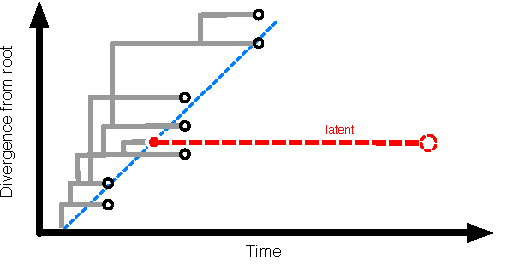
\includegraphics{figures/latency-scheme}
	\caption[Latency Scheme]{ 
	Reconstructing the time that a viral lineage entered a latent state from sequence variation.  
	A dashed line illustrates the linear relationship between the divergence of lineages from the ancestral sequence at the root ($y$-axis) and passage of time since the root ($x$-axis).
	Grey lines represent the reconstructed phylogenetic relationships among these lineages.
	The lineages were sampled (open circles) at three points in time.
	%Above is a time calibrated phylogeny with three taxa, the dotted line in is an example of latency. 
	One of these lineages had become latent at an earlier point in time (red hexagon).
	This lineage subsequently underwent negligible molecular evolution until it was sampled as integrated viral DNA (dashed circle).
	If the relationship between sequence divergence and time is sufficiently linear, then the time that the lineage became latent can be inferred from its sequence, here represented by the thick red dashed line.
	%Sequence A was archived at time $t$, and was collected at the same time as sequence B, at time $t^\prime$ (a drift of $t^\prime - t$ is expected).
	%If the molecular clock assumption holds true, the MRCA is known, and B and C are reliable time-points, then the date at $t$ can be inferred from from the expected amount of evolution for B from the root.
	}
	\label{fig:latenttree}
\end{figure}

\begin{figure}[ht]
	\centering{}
	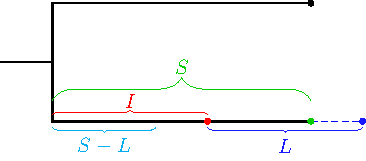
\includegraphics[width=10cm]{figures/latency-model}
	\caption[Latency Model]{An illustration of the latency model. On a tip with branch length $S$, we randomly select a become unlatent period, $U$, and then random select a become latent period, $L$, between the interval $S-U$ and $S$. In the illustration, the red dot represents when the lineage begins to go latent, the green dot represents when the lineage is sampled, and the blue dot represents when the lineage would have been reactivated if it was not sampled. }
	\label{fig:latencymodel}
\end{figure}


\begin{figure}[ht]
	\centering
	\begin{subfigure}[ht]{8cm}
		\centering
		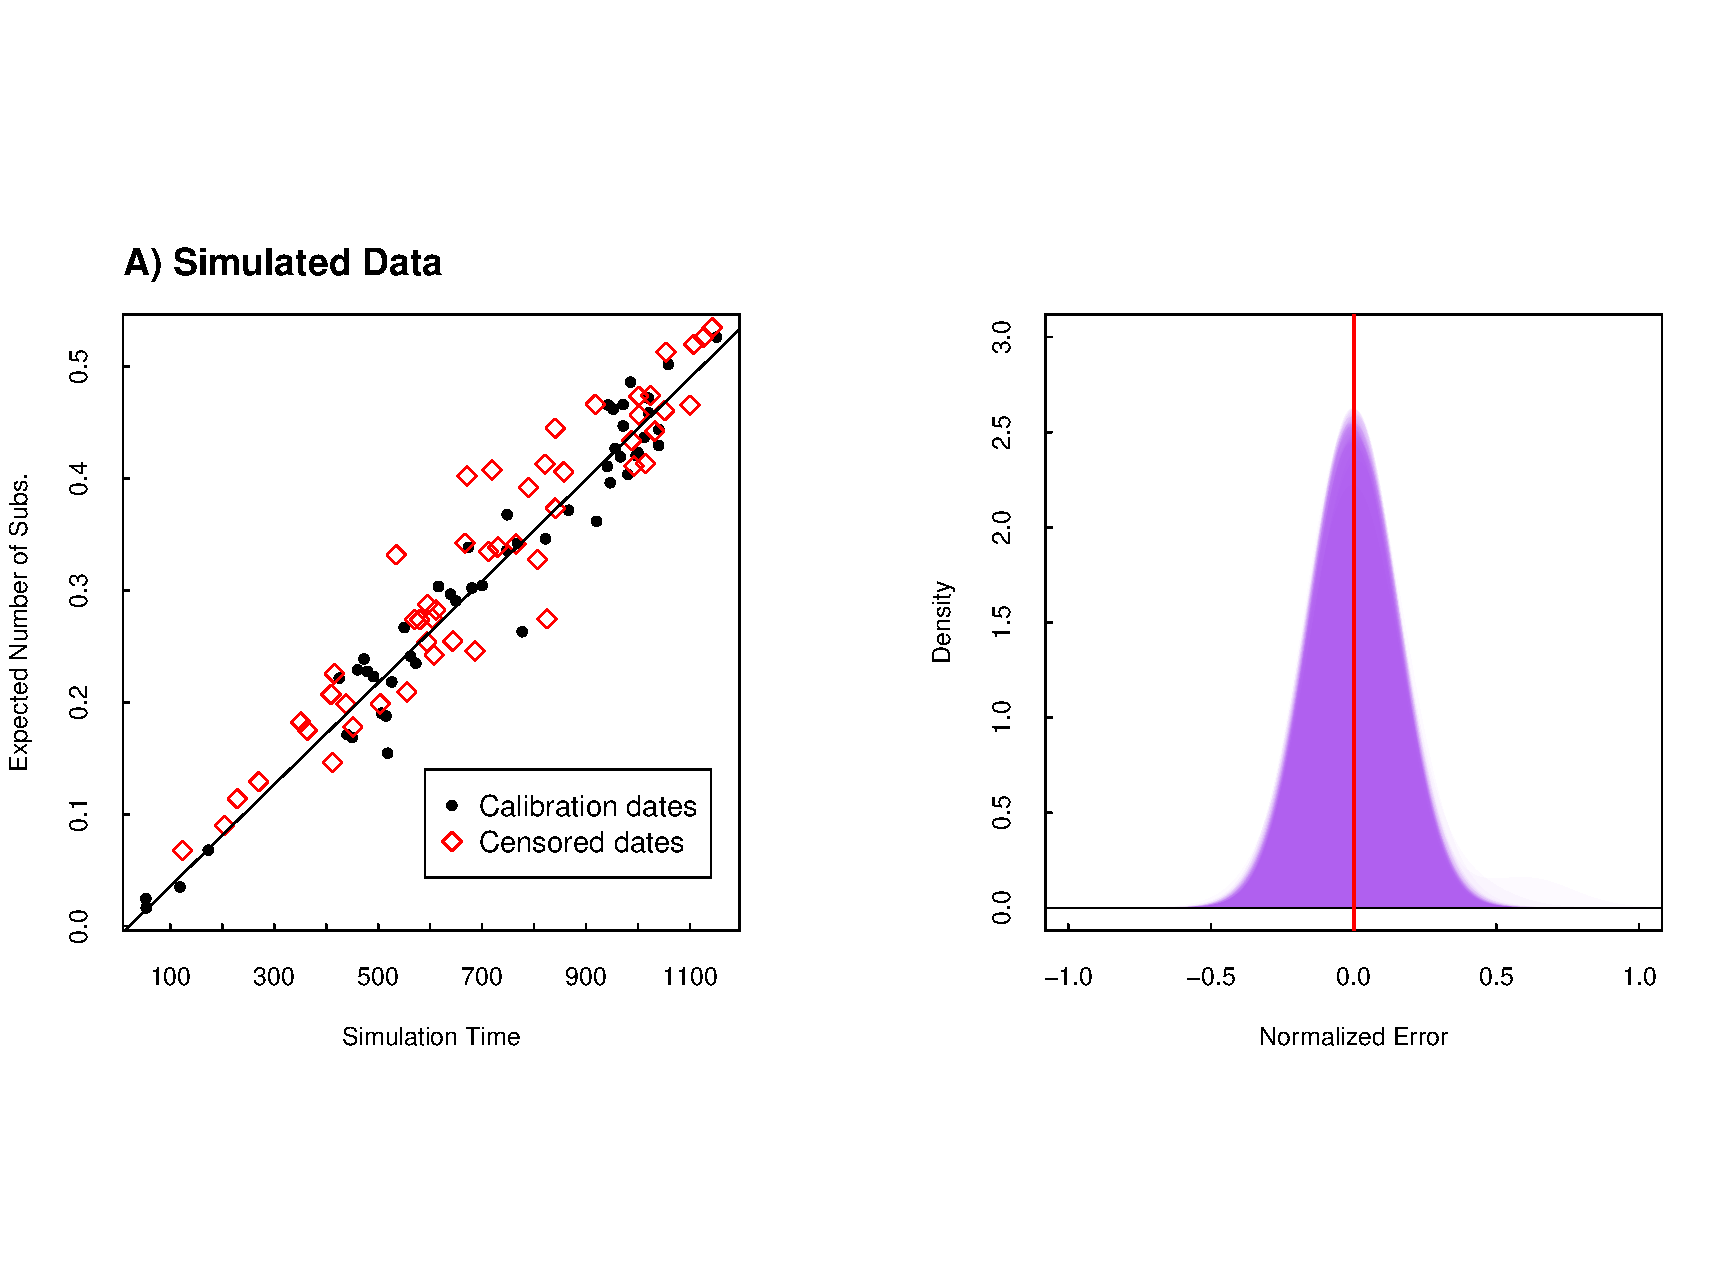
\includegraphics[width=8cm]{figures/simulated.pdf}
		\caption{Simulated data without latency}
		\label{fig:resultssimulated}
	\end{subfigure}
	\begin{subfigure}[ht]{8cm}
		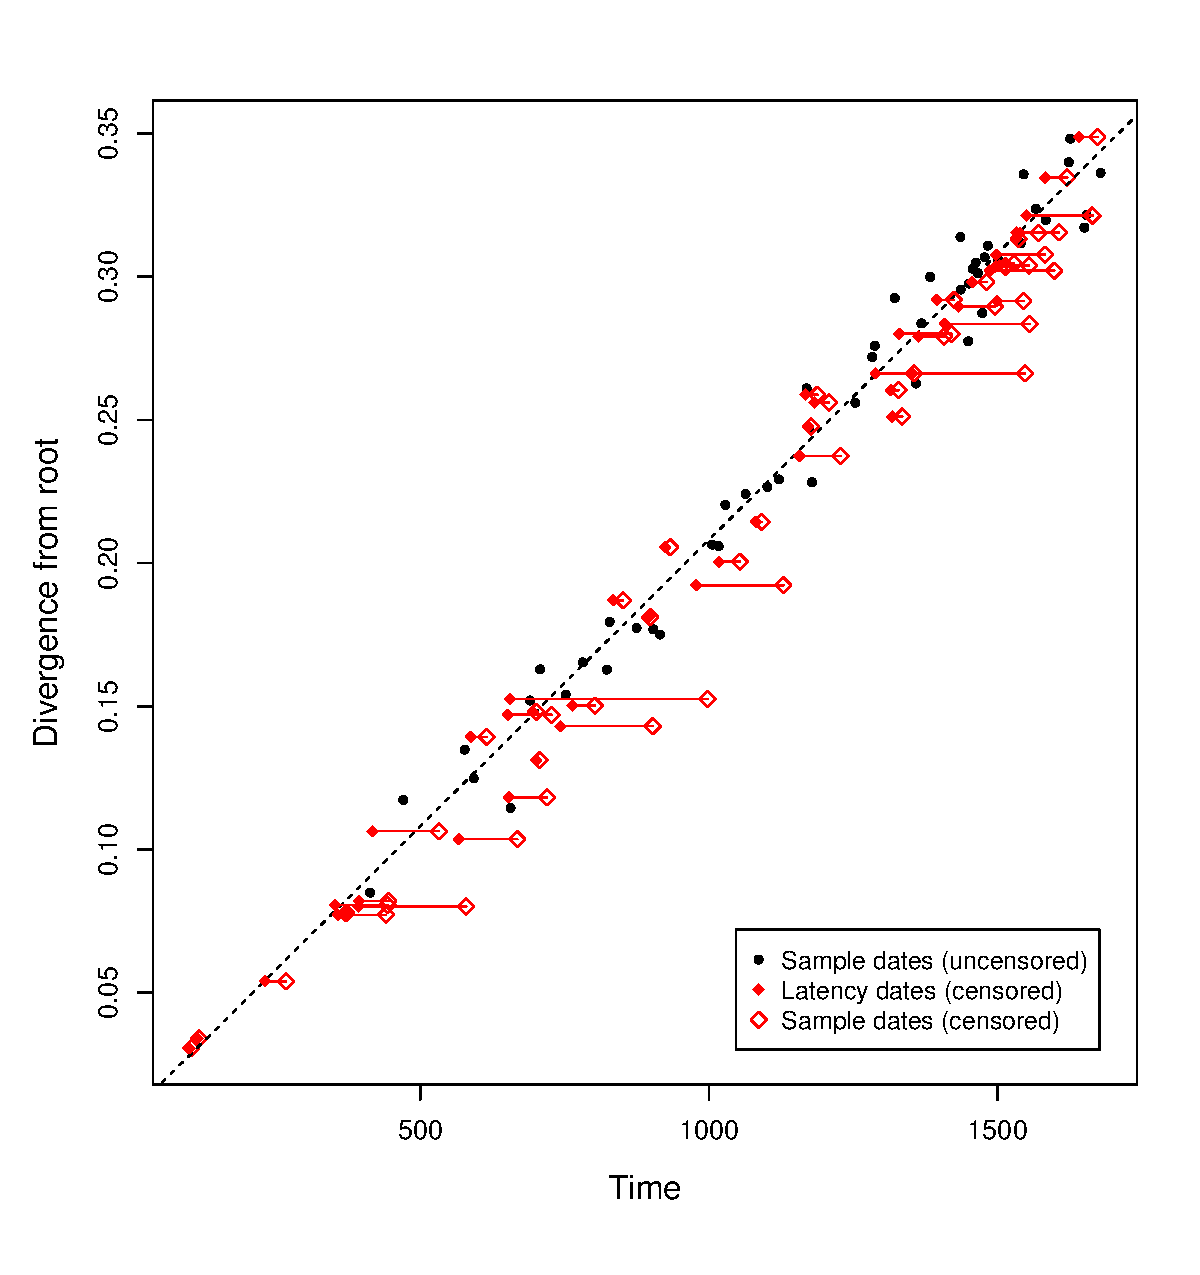
\includegraphics[width=8cm]{figures/simulated_latent1.pdf}
		\caption{Simulated data with latency}
		\label{fig:resultslatent}
	\end{subfigure}
\begin{comment}
	\begin{subfigure}[ht]{8cm}
		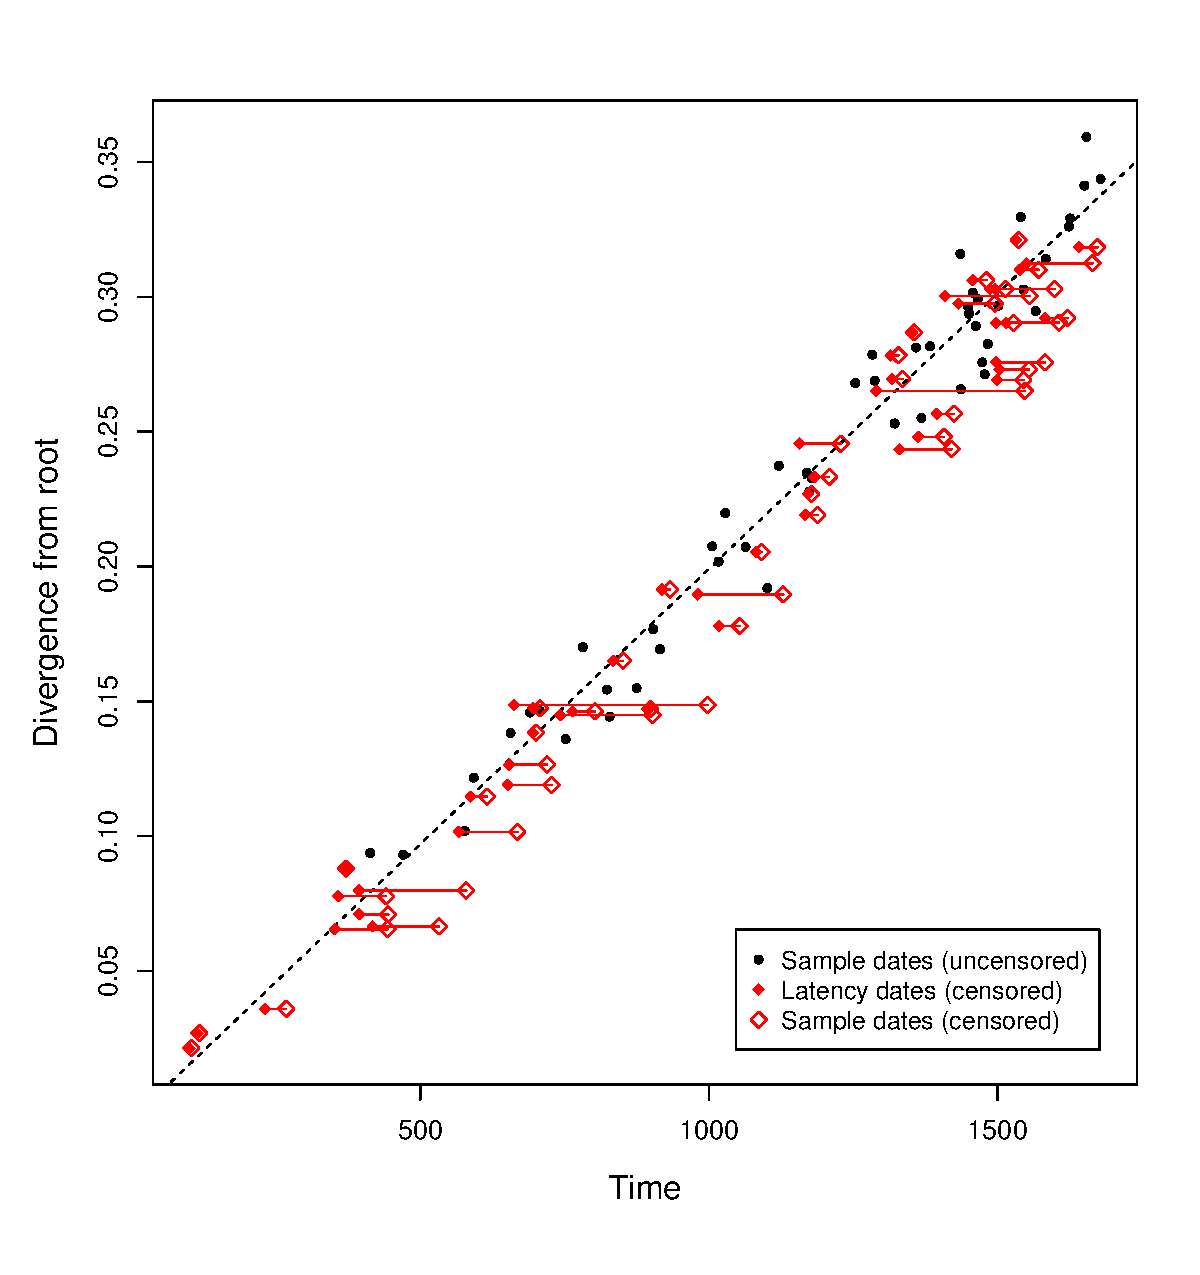
\includegraphics[width=8cm]{figures/simulated_latent2.pdf}
		\caption{Simulated data with latency from the second set}
		\label{fig:resultslatent2}
	\end{subfigure}
\end{comment}
	\caption[Simulated Data]{Plots from the simulated data set of the evolutionary distance vs time. The dotted line is the linear regression.}
%	\caption[Simulated Data]{On the left of each case is a plot of evolutionary distance vs time, the right is the super position of density estimates (of normalized error) for each phylogeny (with kernel bandwidth = $0.15$). The red line on the density plot is the mean error, and the black line is the median error. }
%	Patient: HIV_4
	\label{fig:results1}
\end{figure}

\begin{figure}[ht]
	\centering
	\begin{subfigure}[ht]{8cm}
		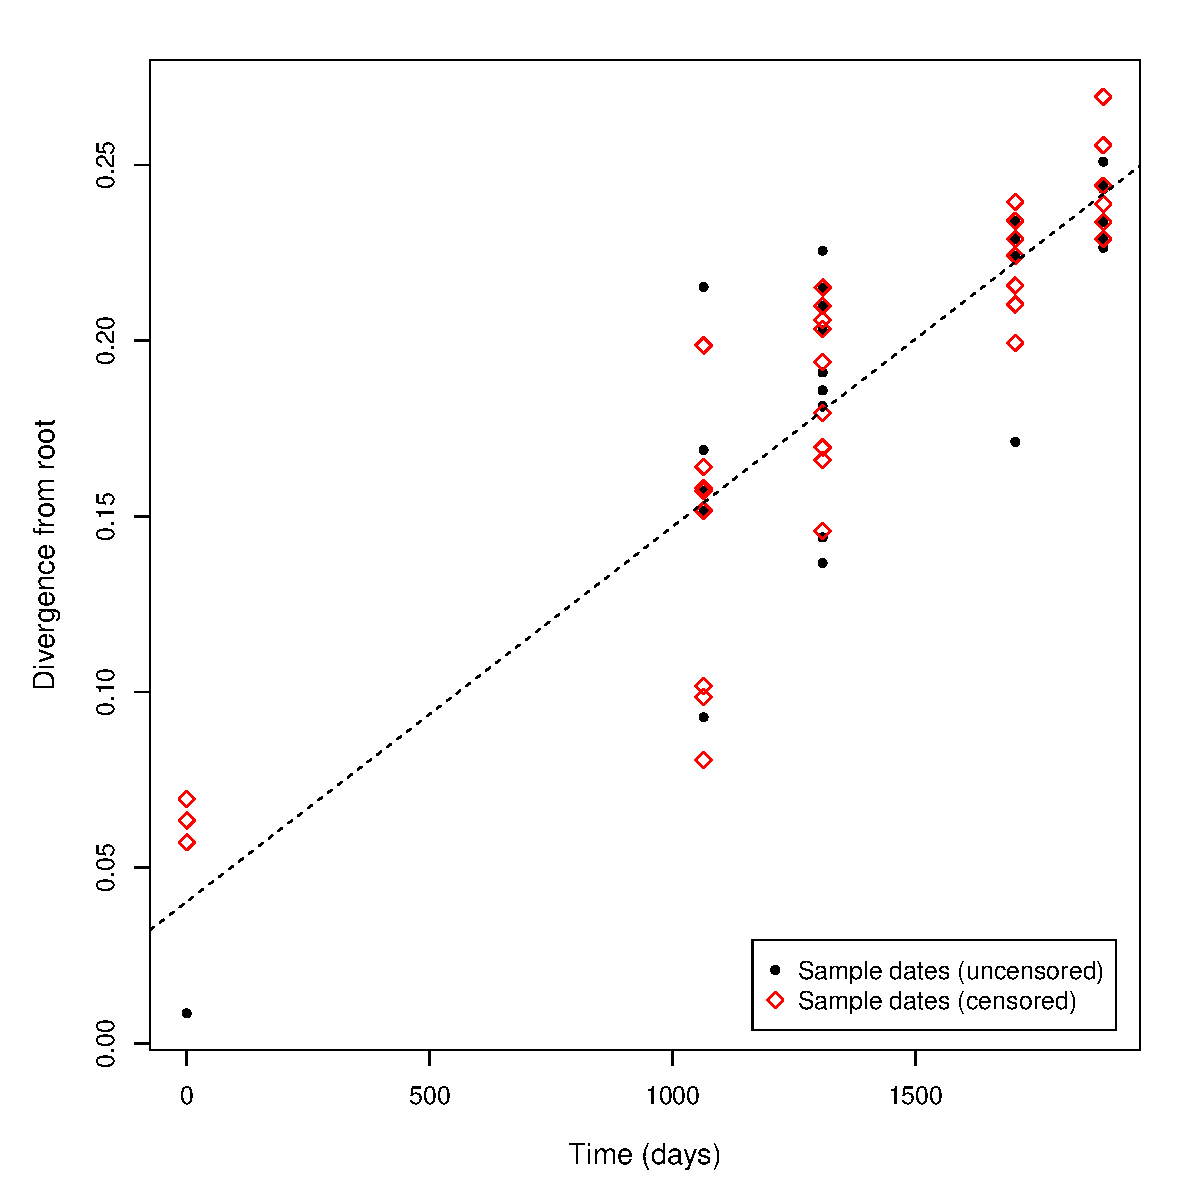
\includegraphics[width=8cm]{figures/ancre.pdf}
		\caption{Patient 2658 from the \emph{plasma} data set}
		\label{fig:resultsancre}
	\end{subfigure}
	\begin{subfigure}[ht]{8cm}
		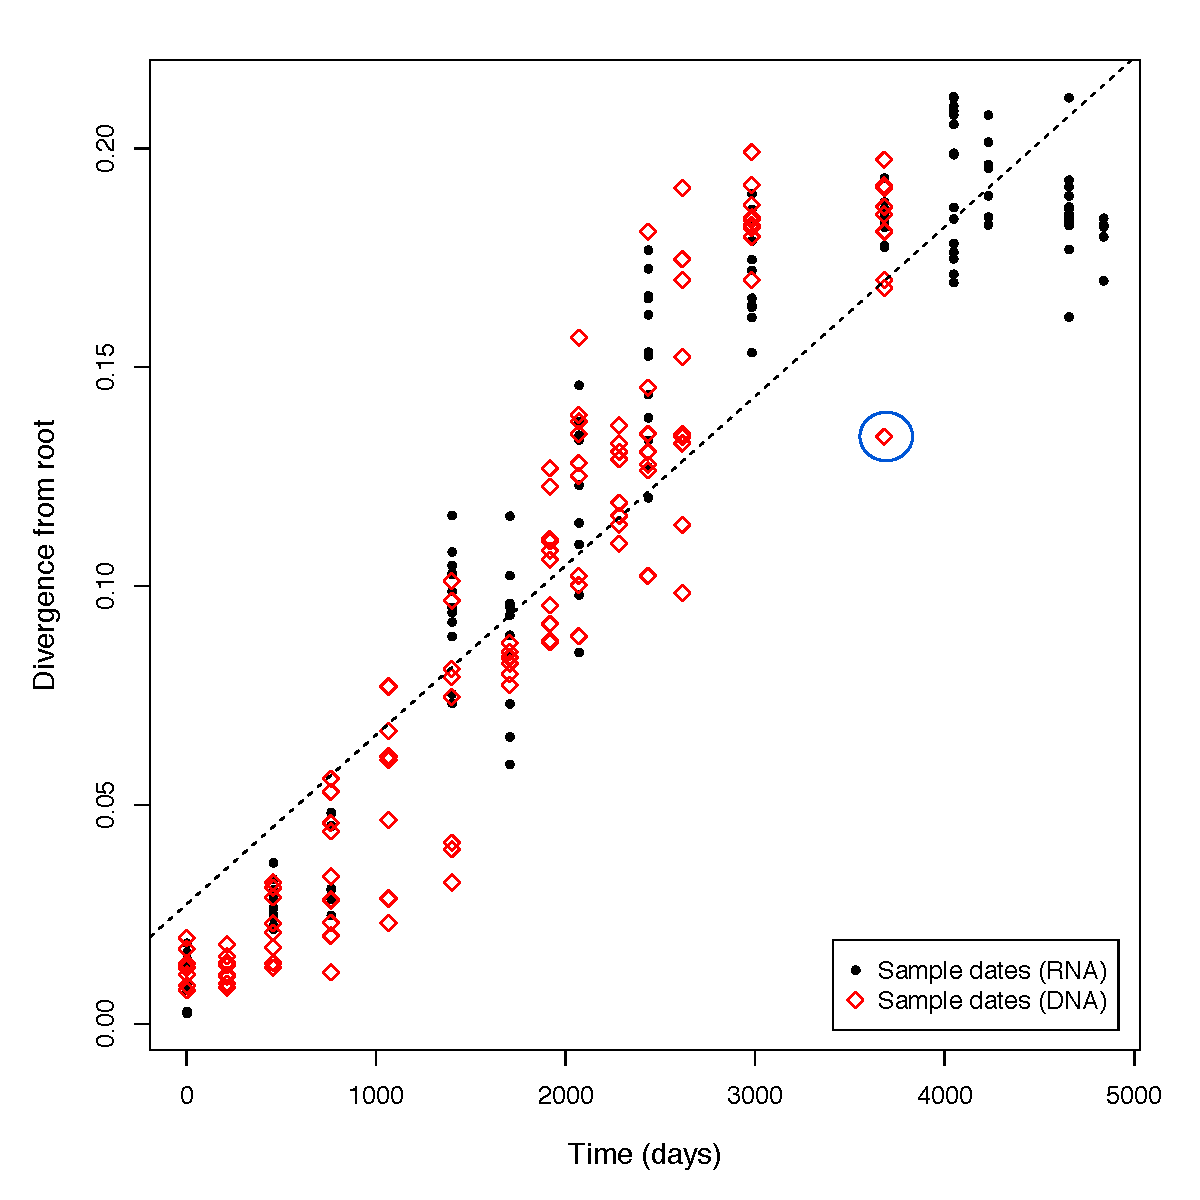
\includegraphics[width=8cm]{figures/lanl.pdf}
		\caption{Patient 13889 from the \emph{mixed} data set}
		\label{fig:resultslanl}
	\end{subfigure}
	\caption[Examples]{As Figure \ref{fig:results1}, except for the real data.}
	\label{fig:results2}
\end{figure}

\begin{figure}[ht]
	\centering
	\begin{subfigure}[ht]{8cm}
		\centering
		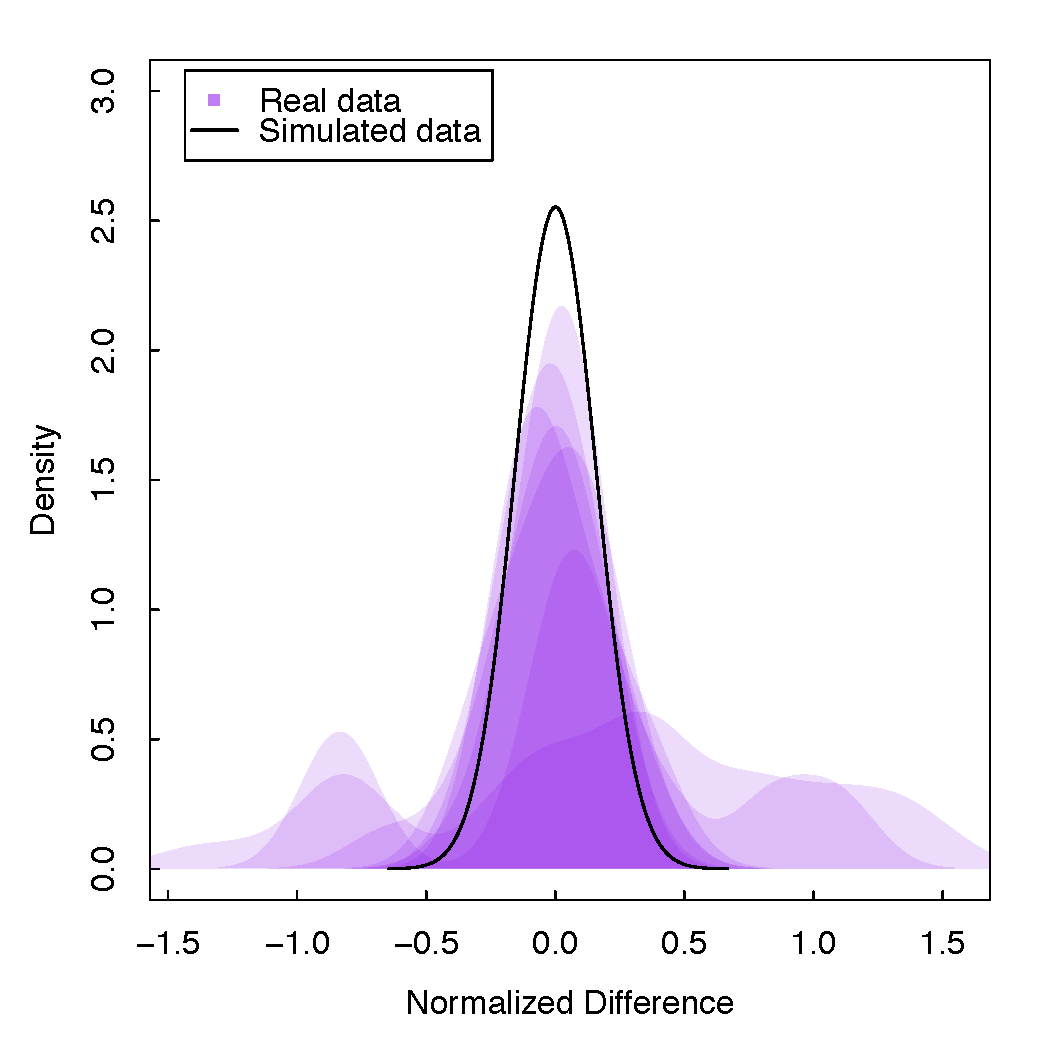
\includegraphics[width=8cm]{{figures/ancre.hist}.pdf}
		\caption{Density of the scaled difference of the \emph{plasma} data set with a solid line representing the density of the difference of the simulated data set without latency.}
		\label{fig:densityancre}
	\end{subfigure}
	\begin{subfigure}[ht]{8cm}
		\centering
		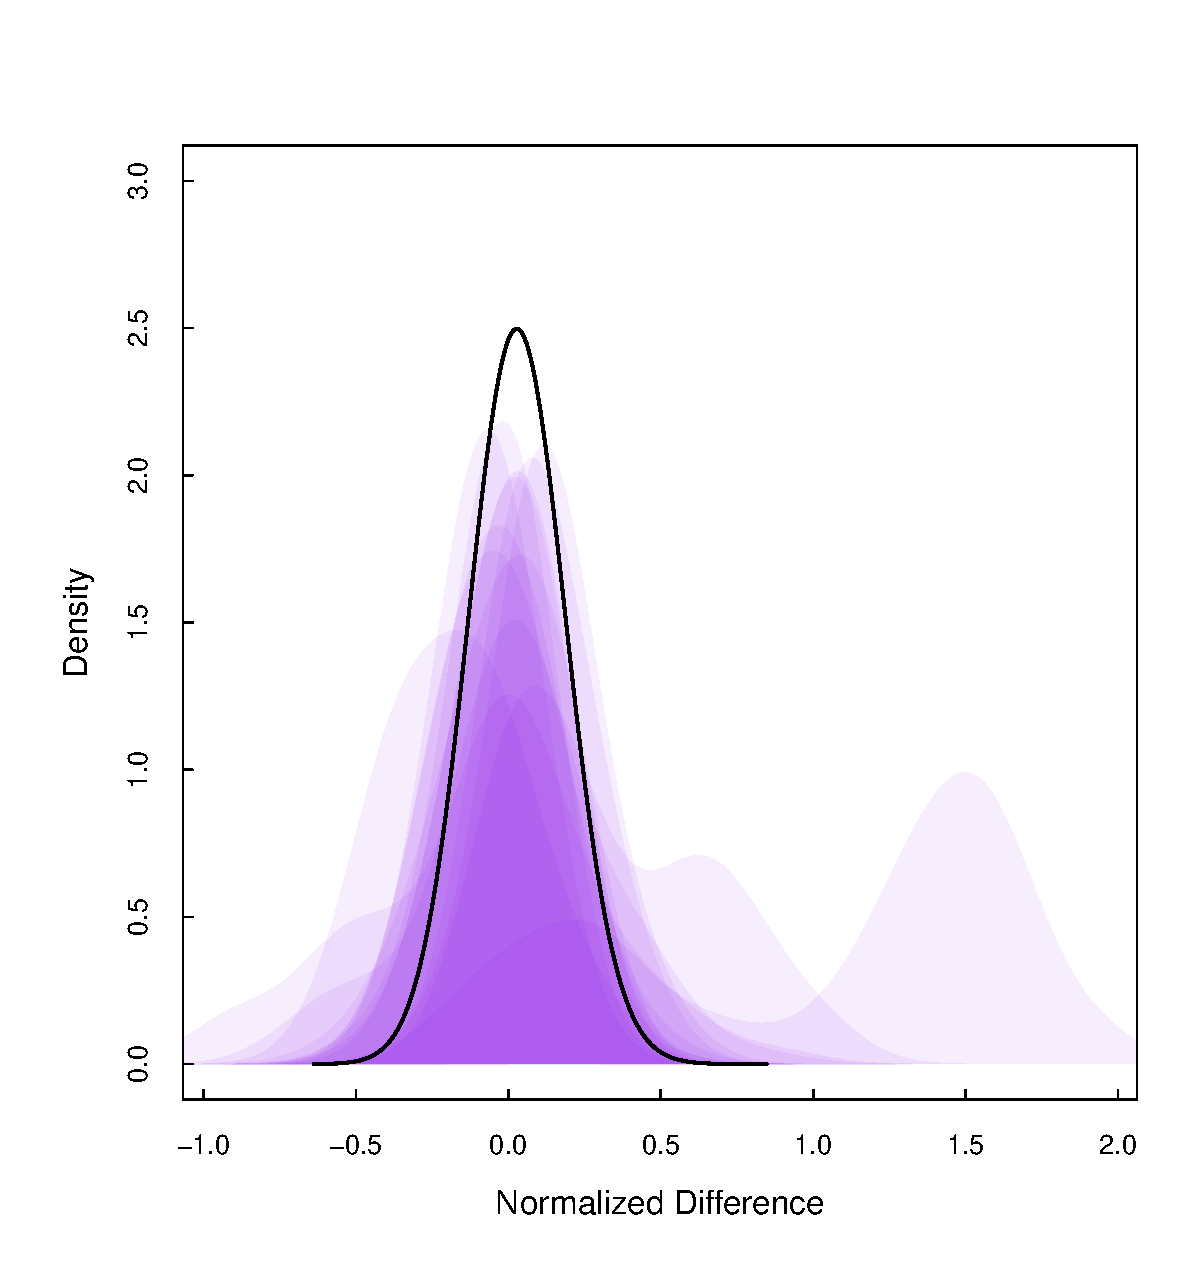
\includegraphics[width=8cm]{{figures/lanl.hist1}.pdf}
		\caption{Density of the scaled difference of the \emph{plasma} data set with a solid line representing the density of the scaled difference of the first set of simulated data set with latency.}
		\label{fig:densitylanl}
	\end{subfigure}
\begin{comment}
	\begin{subfigure}[ht]{8cm}
		\centering
		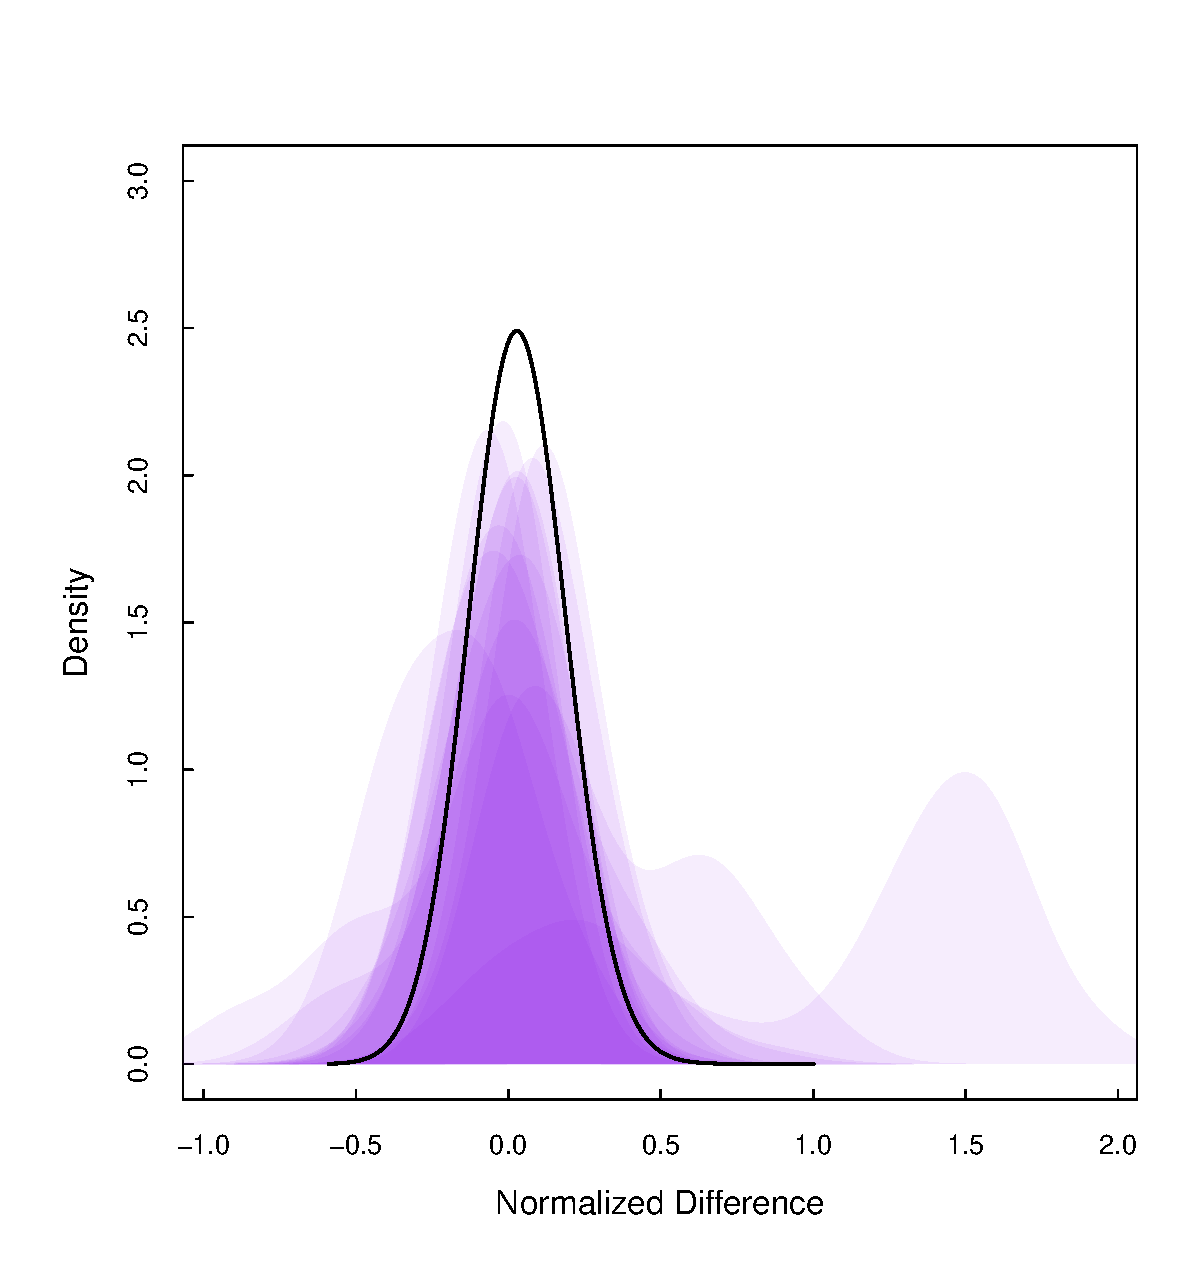
\includegraphics[width=8cm]{{figures/lanl.hist2}.pdf}
		\caption{Density of the scaled difference of the \emph{plasma} data set with a solid line representing the density of the scaled difference of the second set of simulated data set with latency.}
		\label{fig:densitylanl2}
	\end{subfigure}
\end{comment}
	\caption[Difference Density]{The density of the scaled difference. The solid lines represent the density in the simulated data.}
	\label{fig:density}
\end{figure}

\begin{comment}
\begin{figure}[ht]
	\centering
	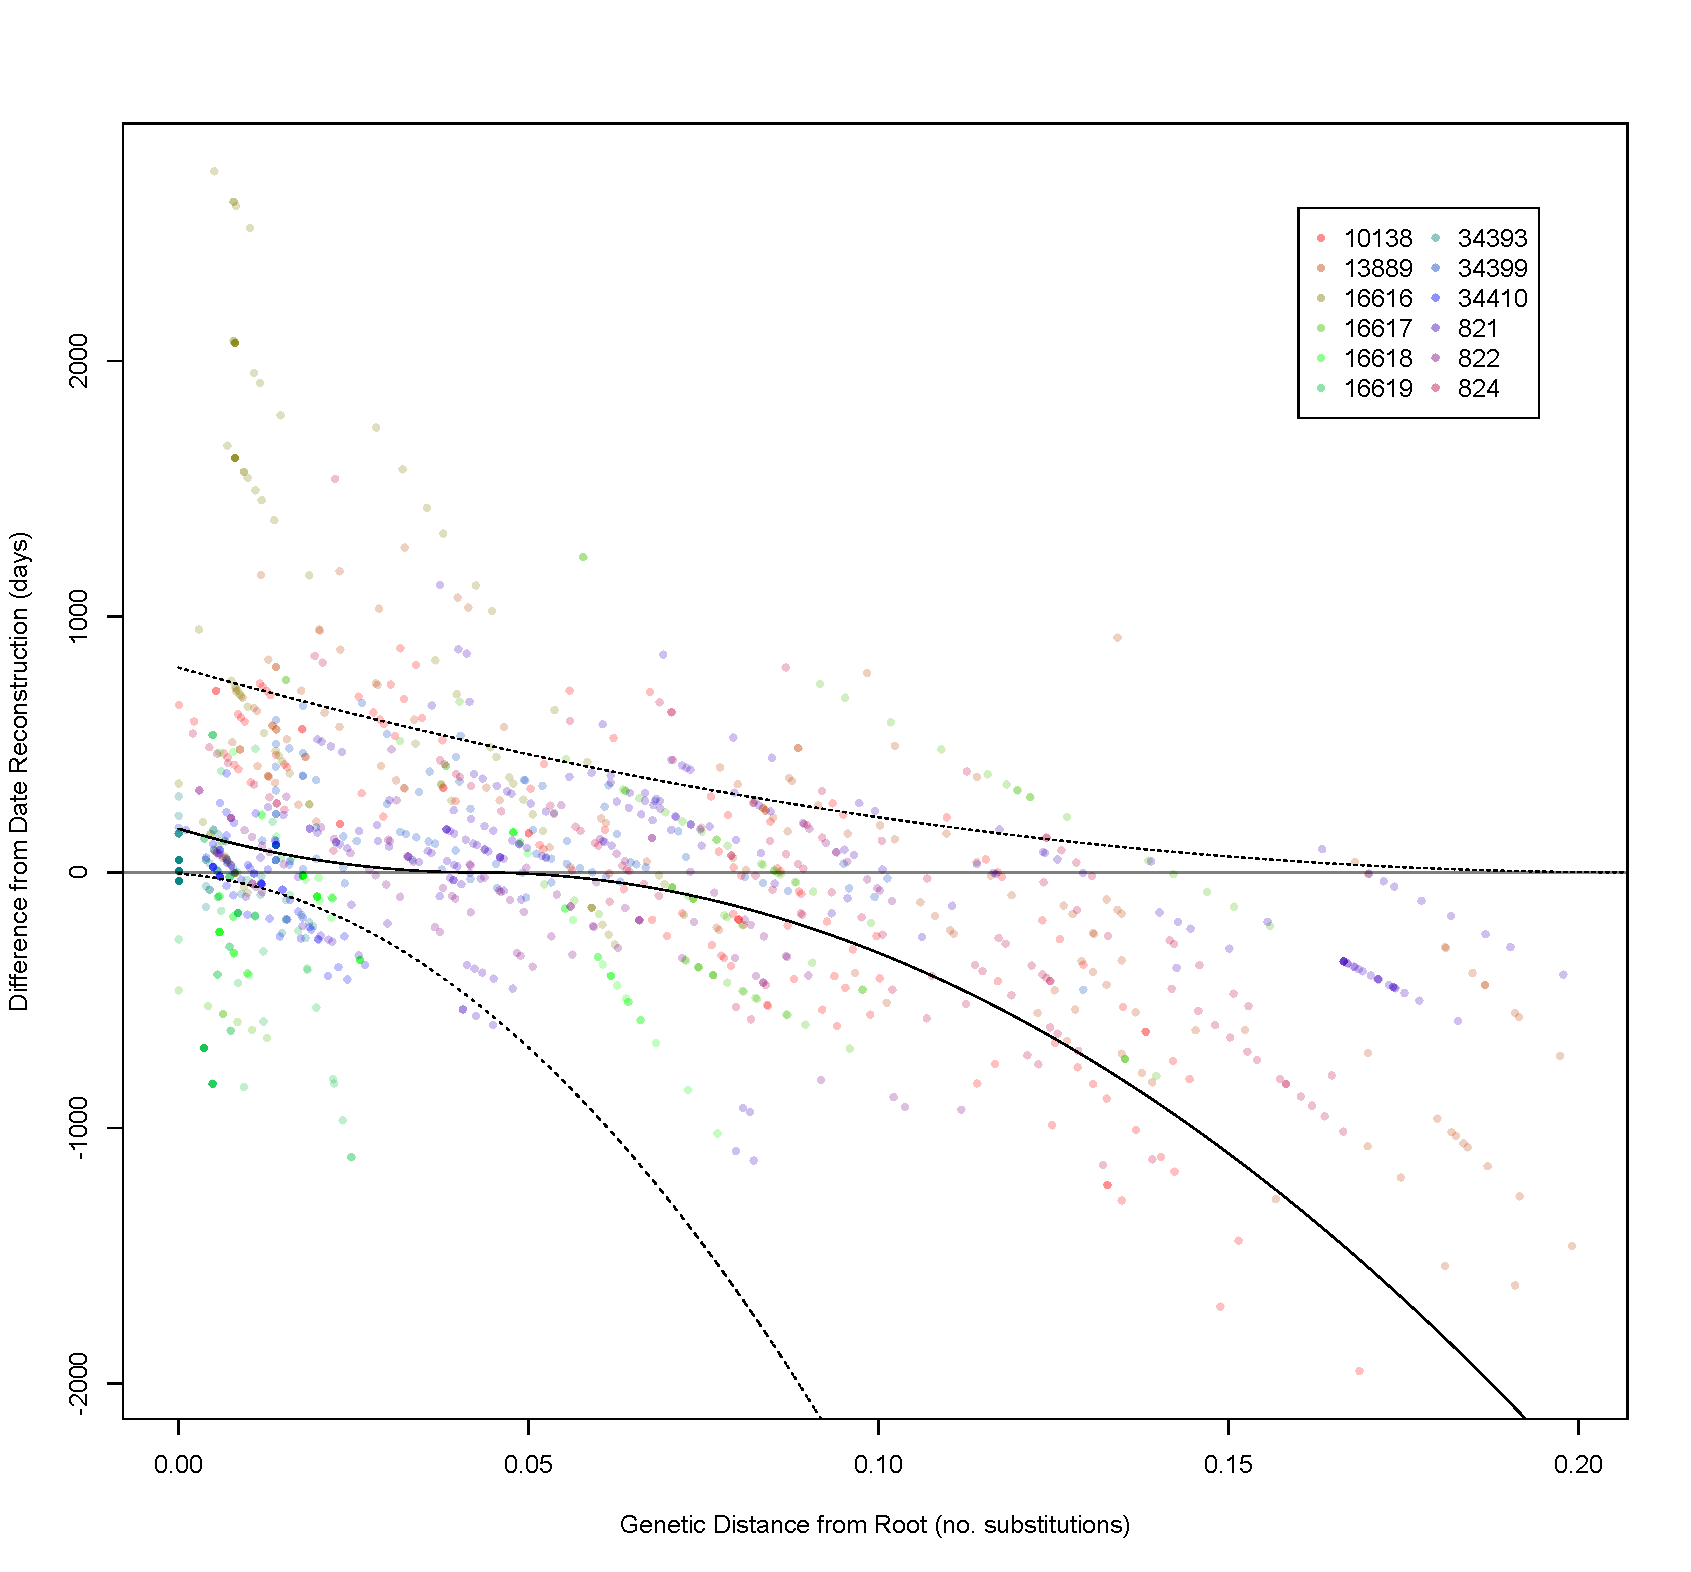
\includegraphics[width=\textwidth]{figures/GLM_plot.pdf}
	\caption[Regression]{A scatterplot of the genetic distance from the root versus the difference from the estimate of the date reconstruction.
	The coloured circles represent the values for each DNA sequence for each subject. 
	The solid black line is the quadratic regression with the mean of the parameters from the mixed effects model.  %The dotted lines are the 95\% confidence interval of the parameters of the quadratic regression.
	}
	\label{fig:glm}
\end{figure}
\end{comment}

%\begin{figure*}[ht]
%	\centering
%	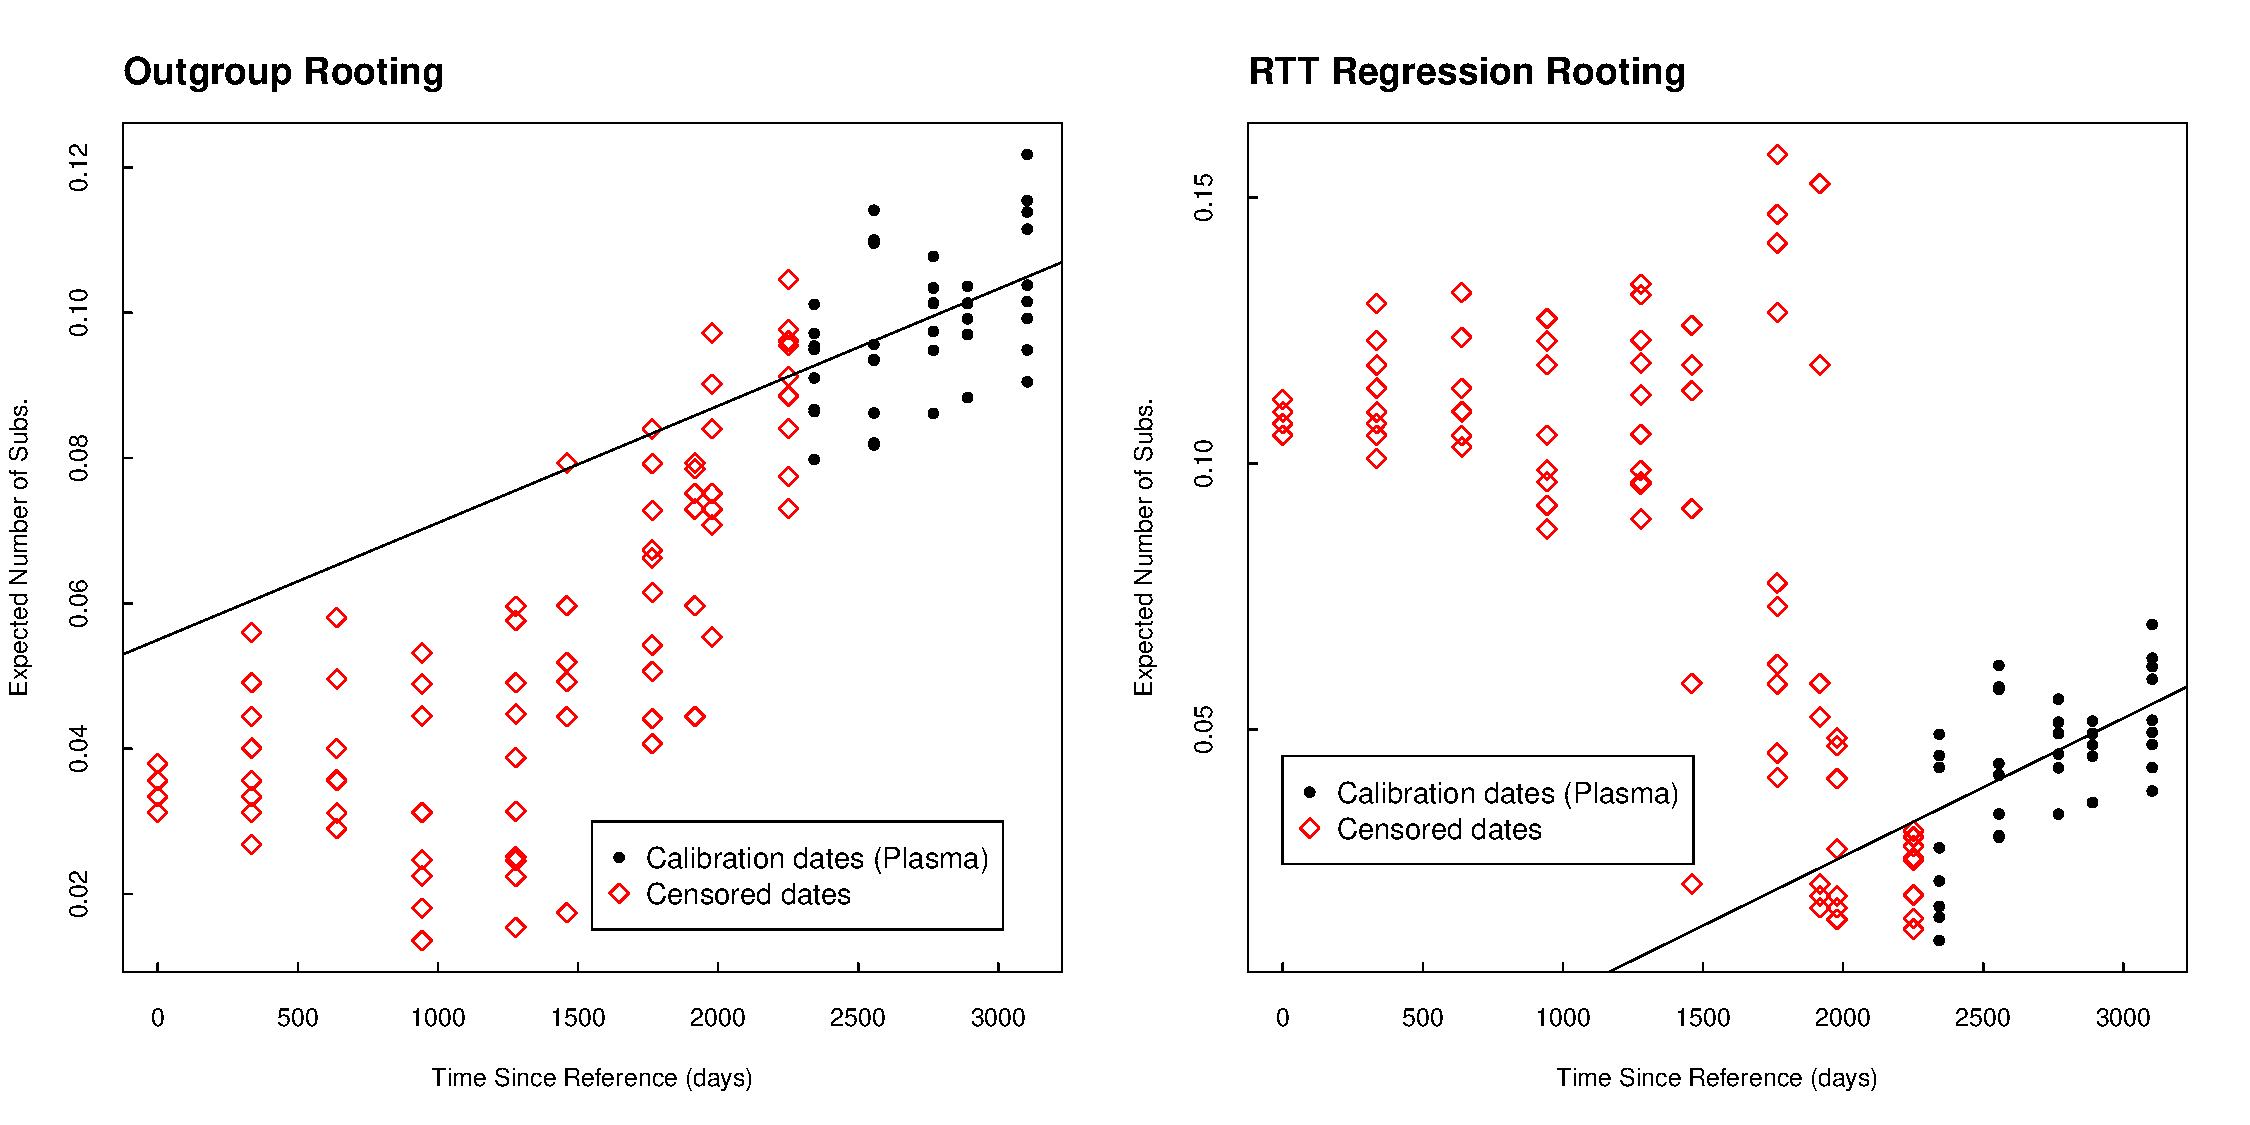
\includegraphics[scale=0.425]{figures/rtt.pdf} \\
%	\caption[Example of bad root]{Root to tip rooting fails due to insufficient temporal resolution at the root}
%	\label{fig:degenerate_example}
%\end{figure*}


\clearpage

%%%%%%%%%%%%%%%  TABLES  %%%%%%%%%%%%%%%

\section * {Tables}

\begin{table*}[!ht]
\def\arraystretch{1.3}%
\begin{center}
\begin{tabular}{llrrrrrrr} 

Reference & Patient ID & \multicolumn{3}{c}{Sequences} & \multicolumn{3}{c}{Time points} \\
 &  & Plasma & PBMC & Total & Plasma & PBMC & Total\\
\hline
\cite{McCloskey14} & 825 & 53 & & 53 & 6 & & 6 \\
& 2658 & 85 & & 85 & 5 & & 5 \\
& 7259 & 29 & & 29 & 4 & & 4 \\
& 7263 & 15 & & 15 & 3 & & 3 \\
& 7265 & 22 & & 22 & 3 & & 3 \\
& 13333 & 40 & & 40 & 4 & & 4 \\
& 13334 & 39 & & 39 & 5 & & 5 \\
& 13336 & 43 & & 43 & 4 & & 4 \\
& 35566 & 93 & & 93 & 2 & & 2 \\
\hline
\cite{Shankarappa99} & 820 &       50 &       87 &      137 &        5 &       10 &       15  \\
& 821 &      76 &      192 &      268 &        7 &       17 &       17 \\ 
& 822 &      32 &       98 &      130 &        3 &       10 &       10 \\ 
& 824 &     100 &      107 &      207 &        7 &        9 &       13 \\
& 10137 &     24 &      106 &      130 &        2 &       10 &       12 \\
& 10138 &     82 &      119 &      201 &        6 &       13 &       16 \\
& 10586 &     16 &      121 &      137 &        2 &       12 &       14  \\ 
& 13889 &    151 &      132 &      283 &       13 &       14 &       18 \\
\cite{Novitsky09}% & 34382 &     37 &        5 &       42 &        3 &        1 &        4  \\ 
& 34391 &     13 &       38 &       51 &        3 &        5 &        6 \\
& 34393 &     25 &       74 &       99 &        2 &        6 &        7 \\
& 34396 &      23 &       46 &       69 &        2 &        5 &        5 \\
%& 34397 &      26 &       25 &       51 &        2 &        2 &        4  \\ 
& 34399 &      61 &       88 &      149 &        5 &        9 &       12 \\
%& 34400 &      54 &       23 &       77 &        4 &        1 &        5  \\ 
%& 34405 &      27 &       29 &       56 &        3 &        2 &        4  \\ 
& 34408 &       5 &       73 &       78 &        2 &        8 &        8 \\
& 34410 &      35 &       60 &       95 &        2 &        6 &        6 \\
& 34411 &      25 &       43 &       68 &        3 &        3 &        6   \\
\cite{Fischer04} & 10769 &    229 &       96 &      325 &       10 &        4 &       11 \\ 
%& 10770 &    190 &       31 &      221 &       11 &        2 &       11  \\ 
\cite{Llewellyn06} & 16616 &     16 &       95 &      111 &        2 &        5 &        5 \\
& 16617 &     16 &       89 &      105 &        2 &        5 &        5 \\
& 16618 &     25 &       75 &      100 &        2 &        5 &        6 \\
& 16619 &     13 &       60 &       73 &        2 &        6 &        6 \\
\hline
\end{tabular}
\end{center}
  \caption{Summary of all the patient data collected from the HIV LANL database in the real data sets --- Patient ID corresponds to the Los Alamos database's Patient ID \citep{LosAlamos}.
   }\label{tab:patients} 
\end{table*}

\begin{table*}[!ht]
\def\arraystretch{1.3}%
\begin{center}
\begin{tabular}{lrrrr} 
Patient ID & $p$-value & Median Difference (days) & RMSD (days) & Scaled RMSD \\ 
\hline
825 & $2.3 \times 10^{-11}$ & -120 & 530 & 0.18 \\
2658 & $2.4 \times 10^{-15}$  & 35. & 220 & 0.12 \\
\badpat{7259 & $0.085$ & 5.9 & 570 & 0.64} \\
\badpat{7263 & $1.00$ & -160 & 190 & 0.77} \\
7265 & $0.0098$ & 18. & 160 & 0.59 \\
13333 & $9.3 \times 10^{-10}$ & 12. & 110 & 0.22 \\
13334 & $2.7 \times 10^{-4}$ & 30. & 140 & 0.19 \\
13336 & $1.9 \times 10^{-12}$ & -40. & 100 & 0.14 \\
35566 & $2.7 \times 10^{-5}$ & 85. & 200 & 0.96 \\
\hline
820 & $4.8 \times 10^{-4}$ & $-3.9 \times 10^{3}$ & $3.7 \times 10^{3}$ & 1.2 \\
821 & $< 2.2 \times 10^{-15}$ & -76. & 340 & 0.14 \\
822 & $< 2.2 \times 10^{-15}$ & 46. & 260 & 0.12 \\
824 & $< 2.2 \times 10^{-15}$ & 45. & 500 & 0.16 \\
\badpat{10137 & $0.031$ & 810 & 890 & 0.32} \\
10138 & $< 2.2 \times 10^{-15}$ & -19. & 560 & 0.18 \\
\badpat{10586 & $0.44$ & $5.2 \times 10^3$ & $7.8 \times 10^{3}$ & 1.7} \\
13889 & $< 2.2 \times 10^{-15}$ & -180 & 628.9 & 0.13 \\
\badpat{34391 & 0.018 & -65.06 & 220 & 0.59} \\
34393 & $2.3 \times 10^{-4}$ & -5.2 & 103.6 & 0.29 \\
\badpat{34396 & 0.15 & -710 & 630 & 1.9} \\
34399 & $< 2.2 \times 10^{-15}$ & -110 & 250 & 0.17 \\
\badpat{34408 & 0.50 & -77 & $1.0 \times 10^{3}$ & 1.9} \\
34410 & $2.1 \times 10^{-6}$ & 16. & 170 & 0.38 \\
34411 & $9.4 \times 10^{-9}$ & -41. & 88. & 0.19 \\
10769 & $1.2 \times 10^{-5}$ & -880 & $2.4 \times 10^3$ & 1.2 \\
16616 & $3.1 \times 10^{-5}$ & -540 & $1.2 \times 10^{3}$ & 0.45 \\
16617 & $1.0 \times 10^{-7}$ & 75. & 440 & 0.17 \\
16618 & $7.7 \times 10^{-12}$ & 110 & 310 & 0.14 \\
16619 & $5.5 \times 10^{-4}$ & 300 & 540 & 0.27 \\
\hline
\end{tabular}
\end{center}
  \caption{Details of the linear models applied to the real data sets. RMSD is the root mean squared deviance. Patients where we were unable to reject the null hypothesis are marked in red.
   }\label{tab:patientserror} 
\end{table*}

\begin{table*}[!ht]
\def\arraystretch{1.3}%
\begin{center}
\begin{tabular}{lrr}
Data set & Total Scaled RMSD & Total Scaled Median Difference \\ % TMD (days) & Median Latency (days)  \\ 
\hline
simulated (no latency) & $4.5 \times 10^{-2}$ & $6.7 \times 10^{-4}$ \\% & $1.3$ & $0$ \\
simulated (extreme latency) & $3.3 \times 10^{-2}$ & $-5.6 \times 10^{-2}$ \\ % & $-70.$ & $90.$ \\
simulated (latency 1) & $6.5 \times 10^{-2}$ & $-2.3 \times 10^{-2}$ \\ % & $-51.$ & $35.$ \\
simulated (latency 2) & $6.7 \times 10^{-2}$ & $-2.3 \times 10^{-2}$ \\ % & $-52.$ & $37.$ \\
\emph{plasma} & $4.4 \times 10^{-1}$ & $2.6 \times 10^{-2}$ \\ % & $23.$  & \\
\emph{mixed} & $3.6 \times 10^{-1}$ & $2.6 \times 10^{-2}$ \\ % & $-41.$ & \\
\hline
\end{tabular}
\end{center}
 \caption{Details of the error metrics of the linear models applied to each data set.
 % Scaled RMSD is the total scaled root mean squared deviance, TSMD is the total scaled median difference, TMD is the total median difference.
 }\label{tab:error} 
\end{table*}

\end{document}
